%----------------------------------------------------------------------------------------
% PACKAGES AND OTHER DOCUMENT CONFIGURATIONS
% WARNING: Don't mess with any of the following unless you know what you are doing.
%----------------------------------------------------------------------------------------
\documentclass[english,12pt,a4paper,openany]{book}
\usepackage{datetime}
\usepackage{tabularx}
\usepackage{makecell}
\usepackage{eurosym}
\usepackage{pbox}
\usepackage{listings}
\usepackage[utf8]{inputenc}
\usepackage[T1]{fontenc}
\usepackage[english]{babel}
\usepackage{amsmath}
\usepackage{amsfonts}
\usepackage{fancyhdr}
\usepackage{amssymb}
\usepackage[dvipsnames]{xcolor}
\usepackage{mdframed}
\usepackage{multirow}
\usepackage{multicol} 
\usepackage{tikz}
\usepackage{graphicx}
\usepackage[absolute]{textpos} 
\usepackage{colortbl}
\usepackage{array}
\usepackage{geometry}
\usepackage{hyperref}
\pagestyle{fancy}
\renewcommand\headrulewidth{1pt}
\usepackage{float}

%------------------------------------------------------------------------------------------------------
%	The following are the RGB values for the official ATU colours.
%------------------------------------------------------------------------------------------------------	
\definecolor{ATUGreen}{RGB}{0, 91, 94}
\definecolor{ATULightGreen}{RGB}{172, 245, 189}
\definecolor{ATUNavy}{RGB}{0, 26, 121}
\definecolor{ATUOrange}{RGB}{255, 121, 30}
\definecolor{ATUPurple}{RGB}{77, 8, 87}
\definecolor{ATUSand}{RGB}{255, 232, 212}
\definecolor{ATUTeal}{RGB}{123, 185, 203}
\definecolor{ATUWarmGrey}{RGB}{200, 190, 191}
\definecolor{ATUYellow}{RGB}{248, 255, 142}



%------------------------------------------------------------------------------------------------------
%	******* CHANGE THE FOLLOWING VARIABLES
%------------------------------------------------------------------------------------------------------	

\newcommand{\reportauthor}{RONAN SHAUGHNESSY} % Change to your name
\newcommand{\projecttitle}{ECHO}
\newcommand{\reporttype}{Minor Dissertation} %Report  type (Project Plan / Final Report)
\newcommand{\supervisorname}{MARTIN HYNES} %Report  type (Project Plan / Final Report)
\newdateformat{monthyeardate}{\monthname[\THEMONTH], \THEYEAR}





%------------------------------------------------------------------------------------------------------	
% WARNING: Don't mess with any of the following unless you know what you are doing.
%------------------------------------------------------------------------------------------------------	
\pagestyle{fancy}
\fancyhf{}
\fancyhead[R]{\textcolor{ATUGreen}{\reportauthor}}
\fancyhead[L]{\textcolor{ATUGreen}{\projecttitle}}
\fancyfoot[L]{\textcolor{ATUGreen}{Atlantic Technological University (ATU), Galway.}}
\fancyfoot[R]{\thepage}

\begin{document}
\begin{titlepage}

\newgeometry{left=6cm,bottom=2cm, top=1cm, right=1cm}

\tikz[remember picture,overlay] \node[opacity=1,inner sep=0pt] at (2.2mm,-165mm){
\includegraphics{images/leftbar.png}}; % Fond changeable 

\fontfamily{fvs}\fontseries{m}\selectfont
\color{white}

\begin{picture}(0,0)
\put(-110,-743){\rotatebox{90}{\Huge{B.Sc. (Hons) in Software Development}}}
\end{picture}
 
\vspace{-10mm} 

\flushright 
\includegraphics[width=100mm]{images/atu-logo-green.png} 

\flushright
\vspace{10mm}
\textcolor{ATUGreen}{
\fontfamily{cmss}\fontseries{m}\fontsize{22}{26}\selectfont
\projecttitle
}
\normalsize
\color{black}

\vspace{1.5cm}
\normalsize
\textbf{By \\ \textcolor{ATUGreen}{\reportauthor}}\\ %Dr. John Healy
\vspace{15mm}
\textbf{for \\  \supervisorname}\\
\vspace{15mm}
{\scshape \today} \\[0.3\baselineskip]
\vspace{75mm}
\Large {\textcolor{ATUGreen}{\textbf{{\reporttype}}}} \\
\bigskip
\normalsize
\textbf{Department of Computer Science \& Applied Physics,\\School of Science \& Computing,\\Atlantic Technological University (ATU), Galway.}\\
\end{titlepage}
\newpage
\tableofcontents
\listoffigures
\listoftables
\pagenumbering{arabic} 

%----------------------------------------------------------------------------------------
%	   ******* CHANGE the Chapters if necessary. Each chapter is encapsulated inside 
%                 its own file. The chapters below are based on the guidelines 
%                 given in the lecture.
%----------------------------------------------------------------------------------------
\chapter{Introduction}\label{chap:intro}
During the course of this year, I will be undertaking a project, which to my hope shall be up to standard of a level eight degree in software and development. Initially I was given the option to be assigned a group, or to work on my own. I have chosen to work by myself, as I feel I can assign myself a good level of scope for the project required. Additionally, I did not wish to be assigned into a group as I had done group work in the past, which worked well however, I never had a say in the application my team was making, this made it really hard to gel into the team, as some design choices were not feasible with too much scope taken into the project. I feel if I operate by myself I can make good design choices and which can be reflected in my project. At the start of the year I coined with working on a project in unity, for example a 3d shooter, with a simple AI of enemies to come and find the player around a medium sized map. However after some thought I imagined the scope would have been too big for one person to take on. My next idea was to create a MERN(Mongo, Express, React, Node) \cite{mern}, CRUD(Create, Read, Update, Delete) \cite{crud} application, to upload memories in a social app setting. This application would also showcase new skills I wished to take on such as testing using cypress, which is a JavaScript testing tool to automatically simulate user behaviour such as button clicks. I decided this application would best suits my skills, as I can engage with new technologies in particular, automated testing. I decided to call the application Echo, I felt this was a unique name as it means to be reminiscent of the past, in which users of the application, may post memories or adventures of their past.

\section{My Idea}\label{section:idea}
My intention is to create a MERN stack application to compliment cypress test automation, with a sign in/register system, sending messages to other users, uploading pictures, liking, and commenting on pictures. In conjuncture to have a fully automated test suite set up using cypress, test cases will also be created to accompany and structure the JavaScript code in cypress, test cases are instructions on how the program should be used, simulating behaviour of a user. My hope is to create a friendly environment where users can upload their travels around the world with friends, or cool hobbies. In addition showcasing new technology for example cypress, in which test automation is used to reduce time from manually testing. Below is a wire frame of how I wish the application to look.

\begin{figure}[h!]
    \centering
    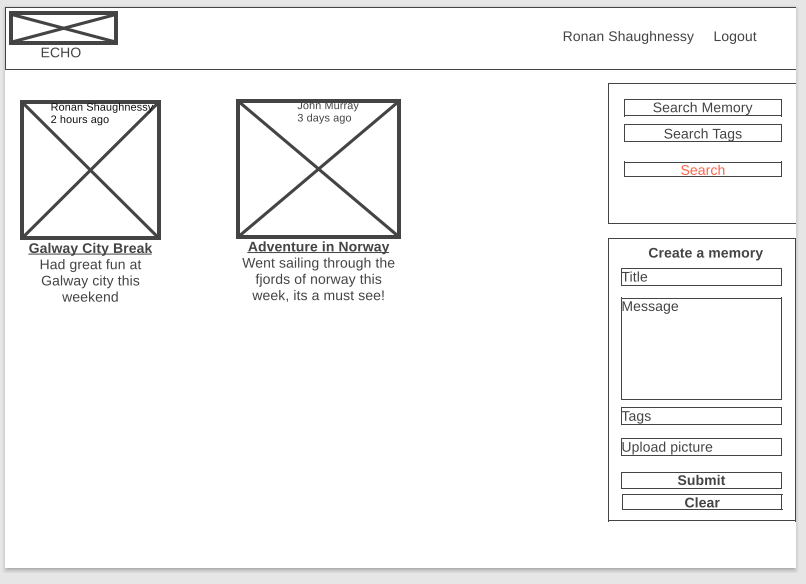
\includegraphics[width=0.78\textwidth]{images/WireFrame.png}
    \caption{Application Homepage.}
    \label{image:AppHome}
\end{figure}

\section{Technology Stack}\label{section:stack}
I plan to use a variety of programming languages I have acquired during the last three years for instance, HTML, CSS, JavaScript, and TypeScript. I decided on MongoDB for my database as according to research I conducted, it stores records as documents, combined with mongoose it can create documents for storing pictures, or any other storage the user will need. I opted for MongoDB over MySQL as I used MySQL often over the last three years, and I wished for a new challenge. I wanted to design the structure of my documents with MongoDB as I find it easier to change Mongo's schema compared to MySQL. I will connect my front-end and back-end using express.js, node.js. Lastly, I will use React for my front-end. I picked React over Angular as during my research I found that React is better for larger web applications as it is more light weight, and I can develop quicker. I feel angular's framework is more rigid and strict combined with the fact React is used more in 2022. Additionally, I wish to improve my skills in software testing, to this end I will employ cypress automated testing to complete testing automatically using TypeScript, and cucumber. Cypress with the aid of TypeScript can create scripts which simulate button clicks, routing to pages etc. This will make testing faster, improving my skills in software testing. I have chosen cypress over selenium as I have never covered cypress, to give me a new challenge and to automate my tests. Following research, I found that cypress manages execution time performance more efficiently than selenium, cypress uses less source lines of code(SLOC) and looks neater when reviewing test cases in the browser \cite{cypresssel}.

\section{Objectives}\label{section:objectives}
The paramount goal is to develop a single-page application, dynamically updating the application, which then allows the user to display photos of their memories and adventures. Moreover to create an application which simulates user behaviour such as button clicks automatically. In order to reach this goal, the subsequent objectives must be present in the application.
\begin{itemize}
    \item To create a dynamic single page application.
    \item The user can register their own account with the application.
    \item The user can sign into their own account once     	registered.
    \item A user is able to post pictures, they wish to share with their friends/family.
    \item Users can search for certain memories using taglines or memory titles.
    \item Users can send messages between each other.
    \item A user is allowed to like a picture, and comment underneath it.
    \item Users can create bio's underneath their posts.
    \item Users should be able to login to their profile and logout.
    \item Designing test scenarios to use in conjunction with cypress automated test tool. 
    \item To have a fully automated test features to verify    the application for commercial use, using test case scenarios designed.
\end{itemize}

\section{Aims}
The purpose of creating the application, what I expect to achieve during the development of the website.
\begin{itemize}
    \item To build a highly pleasing front-end website, which will have a great appearance to please all who visit the application.
    \item To create multiple test scenarios, and have such scenarios fully automated using cypress.
    \item To improve my website design skills using React and JavaScript.
    \item To further my ability using automated testing.
\end{itemize}

\section{Overview}
A brief description of the chapters in this dissertation which illustrate the rationale behind designing this project.
\subsection{Methodology}
This segment describes the work undertaken during the development stage, with particular emphasis on approach to development, validation, testing and tools used to aid development.
\subsection{Technology Review}
This section outlines the technologies which were used in this project, setting up the aforementioned technologies and how the technologies were applied throughout the project.
\subsection{System Design}
This chapter will detail how the project was assembled, how the back-end interacts with the front-end, and will provide a comprehensive description of the overall system architecture.
\subsection{System Evaluation}
This segment will evaluate if the project met the objectives listed in the introduction, and discuss how effectively the system was implemented.
\subsection{Conclusion}
The last chapter examines if the objectives arrayed in the introduction chapter were met, trials which occurred during the development of the project, and how such difficulties were overcome.
\subsection{GitHub Repository}
The GitHub repository for ECHO, my final year project can be found by clicking \href{https://github.com/Rshocks/Final-Year-Project}here.

\chapter{Methodology}
The current section concerns the approaches which were made in undertaking this project, what validation was used, and how units of work were tracked during the course of the project.

\section{Requirements Gathering}
Requirements for this project were gathering in chapter~\ref{chap:intro}, the specific sections where the requirements for the application can be found in these sections, \ref{section:objectives}, \ref{section:stack} and \ref{section:idea}

\section{Planned Approach to Project}
The original planned approach to the application can be seen below in the form of a gantt chart.

\begin{figure}[h!]
    \centering
    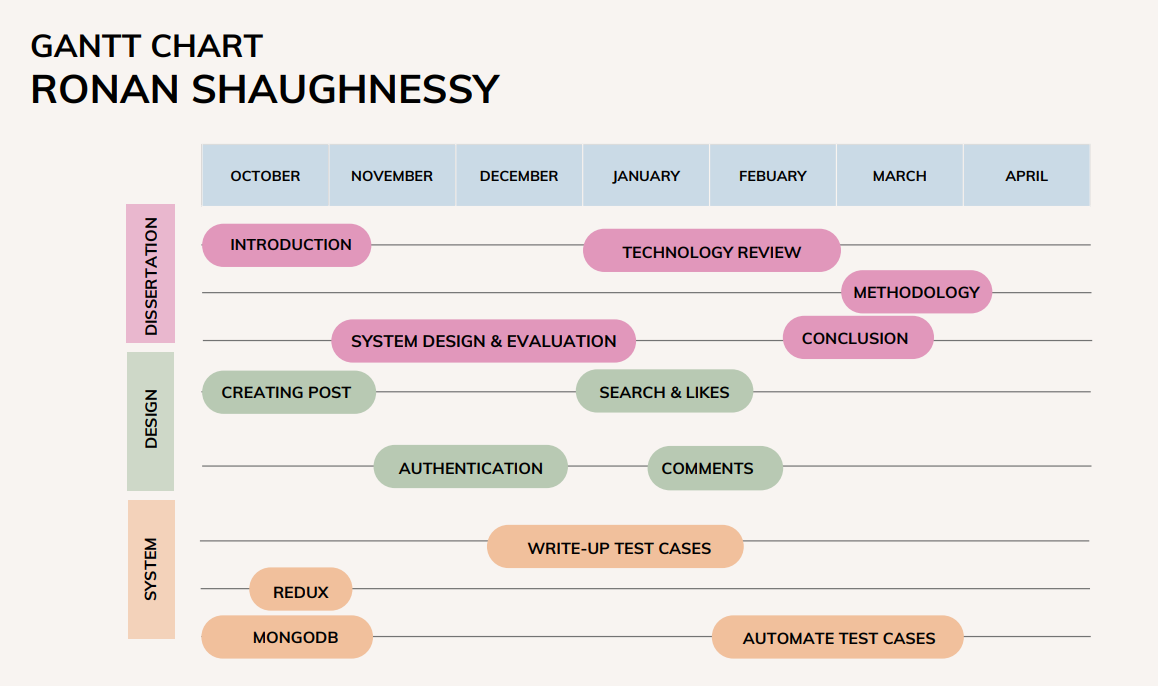
\includegraphics[width=0.5\textwidth]{images/GanttChart.png}
    \caption{Gantt Chart}
    \label{image:GanttChart}
\end{figure}

\newpage
\section{Methodology Approach}
Rather than one single approach, multiple methodologies were used in the creation of the application, Extreme Programming for development, Behaviour Driven Development for testing the application, Jira Software agile tool was also used to track progress alongside GitHub.

\subsection{Extreme Programming}
The approach which was undertaken in order to complete tasks done each week was extreme programming(XP) \cite{akhtar2022extreme}. XP is a agile framework, which takes the agile methodology to the extreme, in short this means shorter sprints combined with more tasks in each sprint. The aims of using XP was to make the most use out of the limited amount of time that was set for the creation of the project, with this in mind maximising all the time during the college year was crucial to the applications success. Lastly XP can handle changes to the requirements smoothly, if the need was deemed high enough for the application.

\subsection{Behaviour Driven Development}
Behaviour Driven Development(BDD) is developing the application, to behave as expected if the application does not function as thought, then work is needed to improve to make the system in order to make it compliant with user behaviour and allow the application to work with ease \cite{abushama2020effect}. BDD was employed to great extent during the testing phases of the application, where test cases needed to be designed based on how the user would interact with the program, in order to assert if it works as planned.

\section{Validation}
Instruments which were used in order to test the application ensuring its appropriate use.

\subsection{White \& Black Box Testing}
Black box methodology was employed using BDD, as BDD takes the role of a user who doesn't care how the applications code base works, only that the application does what is expected. This was used in automated testing of the application, as the Cypress testing tool has no prior knowledge of the internal code base, only simulating user behaviour. White box methodology was employed at a manual test level, as I had a clear idea of the code base which I was working on in order to test the application.

\begin{figure}[h!]
    \centering
    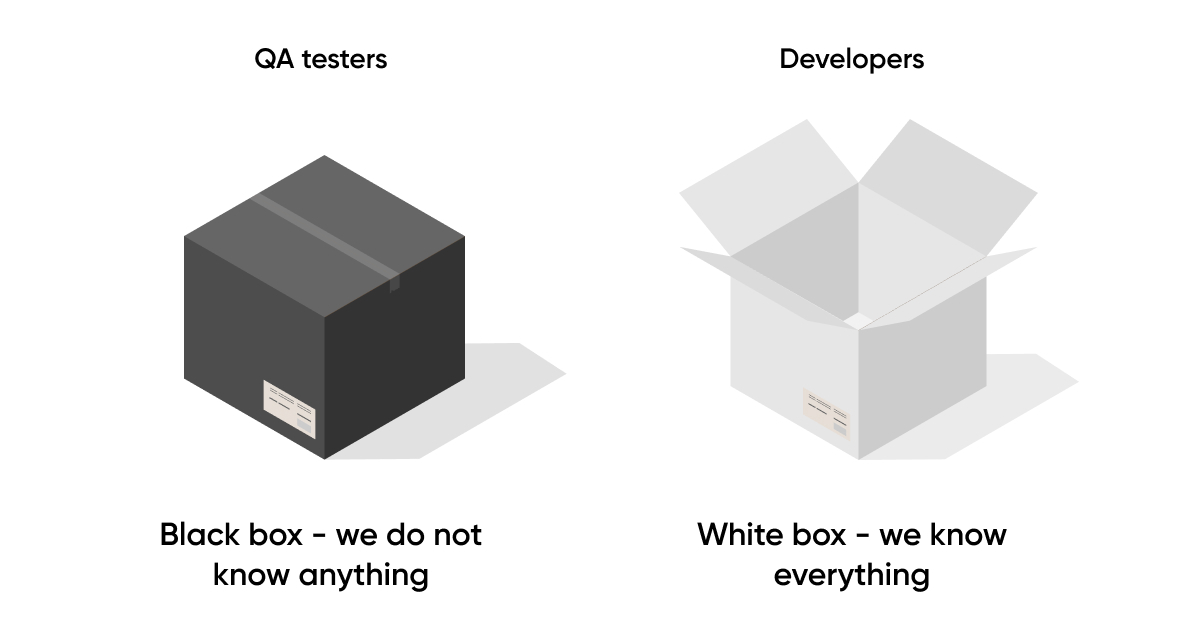
\includegraphics[width=0.5\textwidth]{images/WhiteAndBlack.jpg}
    \caption{White Box vs Black Box Testing}
    \label{image:WhiteAndBlackBox}
\end{figure}

\subsection{Manual Testing}
As previously stated, white box methodology was used during manual testing of the application. When certain restful APIs were called using the application's internal code base, a console.log would be applied to the controller at the back end to determine whether or not there was an error. The aforementioned testing was performed on the application several times throughout the project, using Google's console in the browser to assert if there were errors in the code, this was also accomplished quite successfully with the use of status codes such as the 400, 500 and 200.

\subsection{Automated Testing}
Automated validation was conducted with black box methodology in mind, in which the application would simulate user behaviour for example liking a post once signed in, or creating a post. Automated testing was employed to ensure the front end of the application was working correctly as a user would intend for it to work.

\section{Source Control}
Tools which were used in order to track and manage the software programming.

\subsection{Jira Software}
Jira was used in conjunction with extreme programming to track tickets/tasks. Atlassian stories were created under epics and then brought from the backlog into a new sprint. When a previous sprint finished, tasks were taken into a sprint from the backlog then a new sprint was started, since it was a one man team, each sprint varied in time in custom with XP. At the end of each sprint, the tasks done were evaluated as to how well the aforementioned tasks were completed, after which tickets would be updated if they needed to be brought into the next sprint for improvement, if bugs were found through the use of testing preformed such bugs were logged to be solved in the next sprint, any enhancements which could be made to the application would also be taken into the next sprint.

\subsection{GitHub}
Once a number of tickets were completed during a sprint for example two, then the programming workload would be committed to GitHub, when used in conjecture with Jira it aided to track the projects progress. This was to ensure that the application was always in a stable state, for example if work proceeded after the latest commit, and the code that was being worked on during the latest ticket introduced a breaking bug that halted the application, GitHub could be used to revert the code base, thereby getting the application back to its previous working state. 

\chapter{Technology Review}
This chapter, will discuss the technology used in the projects stack on a theoretical level, detailing features of each piece of technology used in this project.

\section{React}
According to stackoverflow \cite{StackOverflowSurvey}, react.js is the second most common technology for making web based applications at 42.62\%. React was originally launched in May 29 2013, a common misconception is that react is a framework, this is not true, as react is a massive library in which a programmer can make interfaces that revolve around react components \cite{boduch2020react} this along with other features aids to rapid development of a application. React uses the command, create react app to make the application into a framework. React has a seamless development time, making it easier to get applications running using this technology aiding to its popularity over the years \cite{saundariya2021webapp}.

\subsection{React Redux}
The project itself lends a great deal of logic from the redux library of react. These two technologies work very well together and normally go hand in hand \cite{nelson2019developing}. Redux is widely used in this application when state must be changed dynamically without the user noting the change, this greatly supports making a single page application \cite{jadhav2015single}. Redux is best summarized in its key concepts which are employed in the application \cite{caspers2017react}.

\subsubsection{Store}
Store in redux is where the state is stored, this state is then obtained from the store using the getState method, after which the state can be use with the useDisptach method to forward actions.

\subsubsection{Actions}
Actions are responsible for sending the data into the Redux store, actions are the data which alert the store that the state has changed in the application. Redux actions must be a type object, and have other key data so as they are distinguishable to the reducers.

\subsubsection{Reducers}
Redux reducers are viewed as clear functions, such functions take the preceding state and action, then making them inputs thereby returning a new state. A redux reducer script can also be seen as finite state machine, operating on switch statements to switch the state depending on the redux action \cite{holmstedt2019analyzing}.

\subsubsection{Asynchronous Actions}
Lastly redux employs asynchronous actions which can fetch the data from the back-end using redux thunk, after which a response can be handled, and a action can be dispatched so as to update the state of the application. Thunk itself is a middleware, that greatly aids in processing the necessary requests.

\section{Node.js}
Node is a JavaScript run time environment, some of its biggest features include allowing programmers to code in JavaScript on the server side of their application, node can be employed across platforms regardless of OS, and enables programmers to make use of asynchronous programming, so as developers can handle multiple requests in their applications \cite{Node.jsAboutPage}\cite{saundariya2021webapp}. Moreover applications can be launched readily and quickly due to node.js package manager (NPM), greatly aiding a developer to create a application in quick schedule \cite{rawat2020reactjs}. 

\subsection{Node.js Asynchronous Programming}
As eluded to above, Node.js offers asynchronous programming as one of its mainstay features. Such a feature enables a node server to be event driven, and lock free I/O, aiding node in being able to deal with concurrency effectively. Node is able to parse all requests made to it, thereby handling requests in a concurrent fashion using the space execution memory available to it in its one threaded makeup \cite{chhetri2016comparative}.
\begin{figure}[h!]
    \centering
    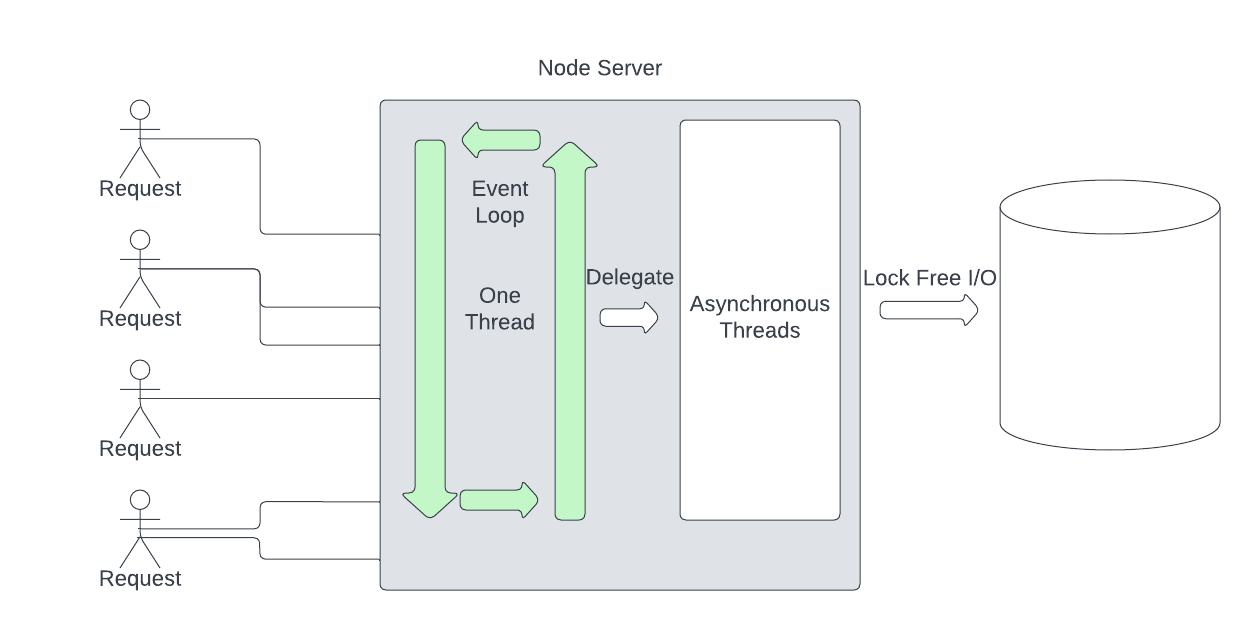
\includegraphics[width=0.8\textwidth]{images/SingleThread.png}
    \caption{Node server makeup using on thread}
    \label{image:SingleThread}
\end{figure}

\subsection{Axios}
Node interacts with react at the front end via HTTP request response, axios helps to streamline this relationship by acting as middleware between node and react, allowing both to send HTTP requests or responses between the server and client sides \cite{saundariya2021webapp}\cite{rawat2020reactjs}.

\section{Express}
Express is a node framework which lends in creating web application, express is normally used in conjecture with node, and can be installed in a application using NPM. Express itself provides an abundance of features for example routing middleware or HTTP capabilities \cite{mardan2018using}.

\subsection{Express as middleware}
Express as a middleware sits between the client and the server, in order to handle request and responses. Express uses functions to take in a request, thereafter such request functions will send back a response, errors when unsuccessful, or relevant data if successful \cite{roomexpress}. In the code snippet below, express is used to log a request and the url to the console. The app.use() method is called, indexing the middleware function, logrequest() is indexed to app.use(), meaning this method will be executed at every incoming request \cite{ExpressMiddleware}. 
\begin{figure}[h!]
    \centering
    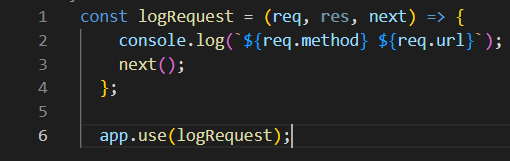
\includegraphics[width=0.4\textwidth]{images/express.png}
    \caption{A brief look at express as a middleware}
    \label{image:express}
\end{figure}
\newline
In the project application of this dissertation an example of how express is used, is to create a request response for users signing into the application.

\subsection{RESTful Express}
Express supports building RESTful APIs for web applications, ways in which Express promotes RESTful usage are, keeping the client side and the server side separate, implementing design patterns for developing web APIs such as aiding in identifying functions to be called for usage, for example get, post, or put. Express can then manipulate such resources over HTTP \cite{REST}, helping to develop an application to be REST compliant by providing robust APIs for handling HTTP requests and responses. Furthermore express promotes REST by handling errors when they occur, or by stating how a user will receive data.

\subsection{Express with HTTP}
Express is built on node.js, using http to access all http functionality, for example get, post being the most common. Express uses http to listen then respond to front end requests \cite{ExpressRouting}. The above-mentioned features allows developers to handle http request through express in the way they see fit, based on the URL and method call, these points make express ideal for making web applications quickly and efficiently.

\section{MongoDB}
Originally developed in 2009, MongoDB is a open source document orientated, NoSQL database which stores, retrieves and manages data for applications \cite{abramova2013nosql}. MongoDB is adeptly suited for numerous applications, for example blog sites which tend to produce a lot of unstructured data, in this case MongoDB is better equipped in dealing with such data in comparison to a RDBMS \cite{agrawal2015survey}. It can be seen as human readable as it stores documents in a JSON like format \cite{calccada2019evaluation}. MongoDB prides itself on having easy to use interfaces, and being able to bring hugely adaptable databases to an application. Beside the features mentioned above, MongoDB ensures acid compliance in their database systems guarantying the validity of data, and uses map reduce as a feature \cite{agrawal2015survey}, which is a data processing model that lends itself to executing actions on sizeable data collections and then assisting in the aggregation of results.

\subsection{MongoDB a NoSQL Database}
There are three types of NoSQL databases, one of which is a document store, MongoDB falls into this category. Document-stored databases are classified as a collection of key-value stores that are then converted into documents and stored in the database \cite{calccada2019evaluation}. One of NoSQL's key features is being able to handle unstructured data to great effect, this is given its rise to popularity in recent years \cite{agrawal2015survey}. Where NoSQL differs from the conventional RDBMS, is that MongoDB's schema is not established in place when compared to a RDBMS, MongoDB will use ID keys in order to retrieve data, as each piece of data is assigned a unique ID key. In reference to the aforementioned, a read/write can only be preformed using the ID key assigned \cite{gyHorodi2015comparative}.

\section{Coding Languages \& Markup Languages}
The below technologies represent the coding languages used in the creation and development of the application.

\subsection{JavaScript}
Developed in 1995, JavaScript or sometimes known as just js, originally created for Netscape 2, although after some time js was preferentially used by Mozilla where it was used to develop web capabilities for Firefox \cite{HistoryJS}. JavaScript is a interpreted language i.e for the computer to understand js, it needs to be complied into something it can understand, normally executable byte code \cite{wilton2004beginning}. With the aforementioned in mind, JavaScript code is interpreted at run time, it is not complied before run time, like for example Java. Attributing to the above, JavaScript is dynamically typed, variables will be assigned at run time, this differs from static typed languages where variables are known at compile time \cite{richards2010analysis}. As such for creating web systems, when a application is running locally, changes can be made to the JavaScript code, then the changes will be shown immediately on the application, provided there are no errors in the code.

\subsection{JavaScript an object orientated language?}
JavaScript is a object orientated language however, js is used more as object based, rather than upholding the principles of object orientated programming. JavaScript as a language promotes the use of being able to change or being agile, as the above mentions js is weakly typed, interpreted, and variables could be removed or added at run time \cite{theisen2019programming}. While js is a object orientated language it is normally not used in such a way, TypeScript a offshoot of JavaScript, is popularly used to adhere with oop principles, which in of itself is a superset of JavaScript.

\subsection{TypeScript}
TypeScript is a superset of JavaScript, this means that TypeScript can understand all JavaScripts syntax and capabilities \cite{cherny2019programming}. TypeScript does more to uphold the principles of object orientated programming, by bringing in classes, interfaces, and is statically typed \cite{bierman2014understanding} catching errors before run time, in many ways TypeScript looks at what JavaScript doesn't do well, then adding features to JavaScript to aid developers. TypeScript does not have a interpreter, instead it compiles to JavaScript as browsers cannot understand TypeScript \cite{jansen2016typescript}. With the above facts in mind, TypeScript is normally used now in favour of JavaScript, as if a person learning web development for the first time, TypeScript uses classes more frequently, and it statically typed language making it more familiar to new comers when compared to JavaScript. Moreover it can be used quite avidly by programmers who use JavaScript as TypeScript understands JavaScript, as it only adds to JavaScript features.

\subsection{TypeScript vs JavaScript}
Below, is a code snippet of TypeScript as a class vs JavaScript as a class, as shown below TypeScript has variables brought in before the constructor i.e variables are known before run time, when compared to JavaScript the variables let person = new Person("Alice", 30); are only assigned during run time.
\begin{figure}[ht]
\begin{minipage}[b]{0.5\linewidth}
    \centering
    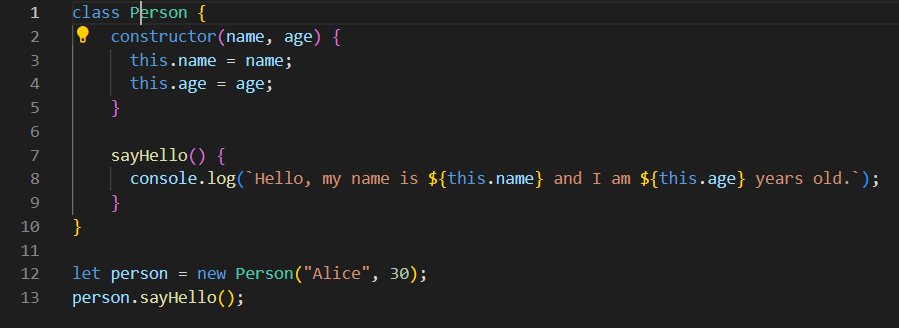
\includegraphics[width=\linewidth]{images/JavaScript}
    \caption{JavaScript as a class}
\end{minipage}
    \hspace{0.5cm}
    \begin{minipage}[b]{0.5\linewidth}
    \centering
   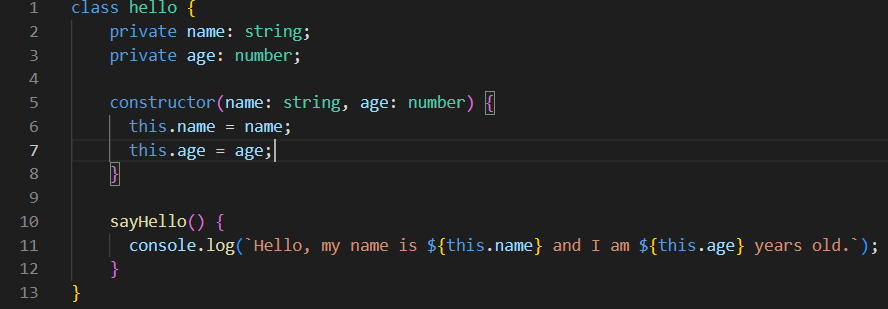
\includegraphics[width=\linewidth]{images/TypeScript}
    \caption{TypeScript as a class}
\end{minipage}
\end{figure}

\subsection{JSX}
JavaScript syntax extension or JSX, which like TypeScript is a addendum to the already established JavaScript. JSX allows developers to outline Reacts object structure into syntax that is comparable to HTML. Simply put JSX, is an XML related addition, allowing programmers to write JavaScript that can appear as a HTML like, and then have it returned as a component in React
\cite{JSX}.

\subsection{HTML}
Hyper Text Markup Language (HTML) is a markup language which is used in representation of web applications. HTML is crucial in any web development as it details the architecture of a web application i.e it explains how the application should be rendered, however the application need not be written in HTML, as it is unable to write functions or carry out complex tasks when compared to JavaScript \cite{minnick2020responsive}.

\subsection{CSS \& Material-UI}
Cascading Style Sheets (CSS) can be closely aligned with the use of HTML or other markup languages, CSS like HTML is also used in changing how a web application is presented, although unlike HTML, CSS tells the application what color, layout or general style elements of the web page should be using \cite{geneves2012analysis}. The creation of pleasing designs can be employed quickly using a CSS framework Material-UI, which follows googles material design patterns, Material-UI comes with existing React components, for example SVG icons, uniformity in displaying forms or navigation bars, and other features. Material-UI can help developers worry less about the look of a application when compared to using normal CSS, as Material-UI will handle most of the aesthetic of the application \cite{nguyen2022building}.

\subsection{JSON}
JavaScript Object Notation, allows programs to represent JavaScript objects in plain text, JSON is used to serialize and parse objects over the network, normally between the front end and the back end. However this comes at a price as the plain text used, are much larger in size when compared to their binary equivalent, therefore parsing must be preformed on both sides for example in client side and server side \cite{JSON}.

\subsubsection{JSON Web Token}
Web tokens are used to identify if users are verified on certain systems for instance, if a user signed into Facebook, a web token would be assigned to them, asserting a authenticated user \cite{JWT}. A JSON web token uses a JSON object to assert safety between two parties normally the user and the client or application the user wishes to use \cite{jones2015json}. Authorization is the most regular use of a JSON web token, when a user is logged into Facebook for example, they will then be able to avail of the activities which Facebook advertises, using their JSON web token which is stored in local storage, all of which is hidden from the users view \cite{JWT}.

\section{Cypress}
Cypress automation test tool is a relatively new web automation tool only being released in 2017. Cypress is a client side testing tool created for web applications, Cypress greatly encourages Behaviour Driven Development, building tests side by side while creating a web application, then asserting such tests pass as development advances \cite{WhyCypress}.

\subsection{Cypress Architecture}
Cypress is often contrasted with Selenium, although the two testing tools are architecturally different. Cypress is built using Node.js, and comes in its own npm module to be installed locally, then running npm to open cypress in a browser window in order to open the application the developer wishes to test \cite{taky2021automated}. Altering web traffic at will, is how Cypress performs operations at the network layer. This gives Cypress the opportunity to change what goes into and out of the browser, allowing Cypress to also adjust code that could cause glitch's or errors in the browser's automation \cite{WhyCypress}, resulting in a smother testing experience, enabling the engineer to obtain accordant outcomes \cite{pelivani2022comparative}. As Cypress is installed into a developers local machine using node, it allows the automation to use the local operating system in order to make use of the camera for taking screenshots of failing or passing tests, and recording videos of the automated test suite.
\begin{figure}[h!]
    \centering
    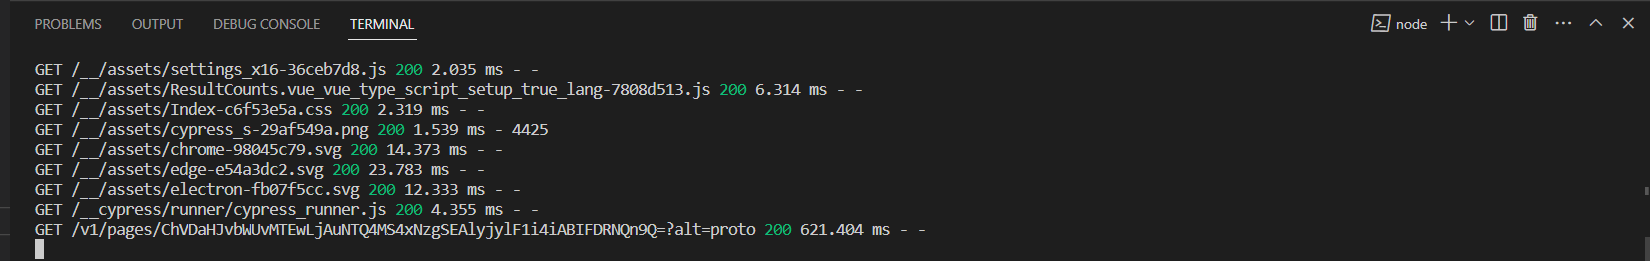
\includegraphics[width=0.8\textwidth]{images/CypressAndNode.png}
    \caption{Node running the server side for Cypress}
    \label{image:CypressAndNode}
\end{figure}
\begin{figure}[h!]
    \centering
    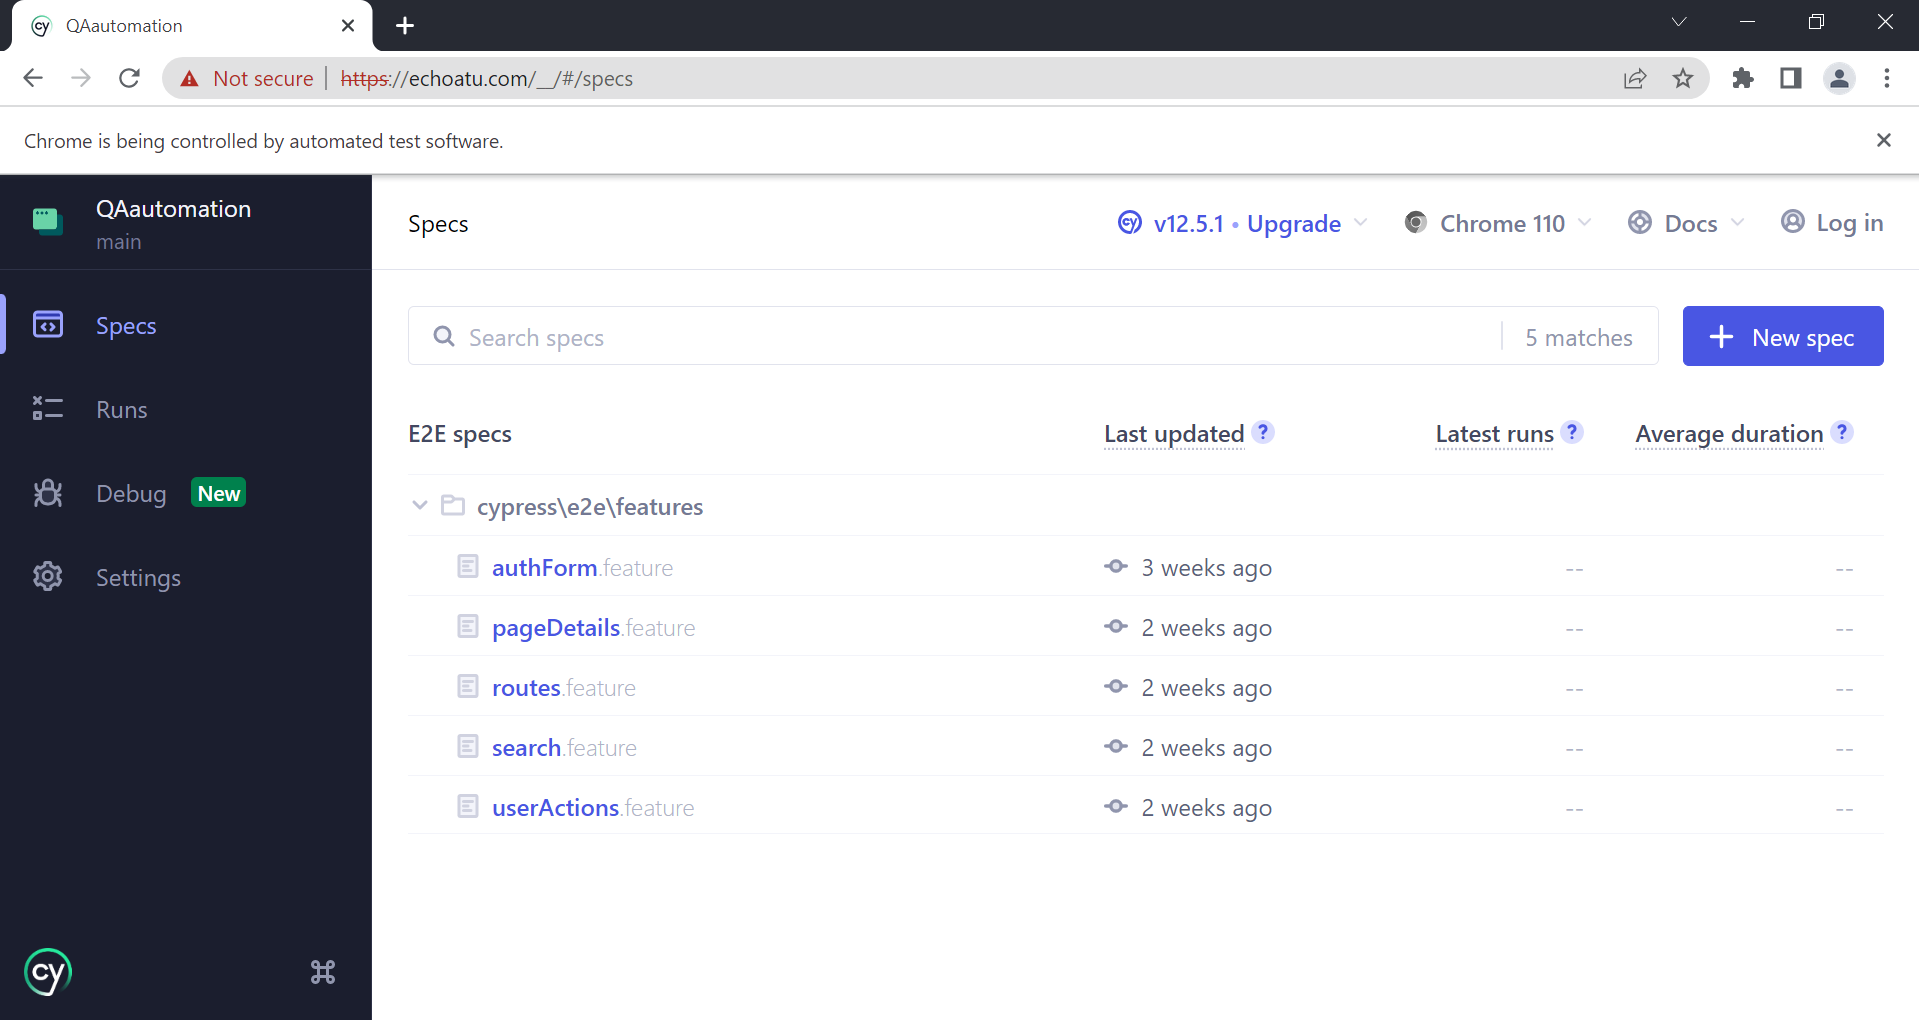
\includegraphics[width=0.5\textwidth]{images/BrowserCypress.png}
    \caption{Cypress running in the browser supported by node.js}
    \label{image:BrowserCypress}
\end{figure}

\subsection{Cypress Features}
Cypress contains a number of capabilities for example Cypress uses the wait command at will in order to wait for the DOM to load in correctly, this is needed greatly as Cypress tests sometimes preform blindingly fast, although if a test engineer wishes for extra time to be applied the cy.wait command can be hard coded in \cite{SwitchCy}. JavaScript is the predominate coding language used in Cypresses testing framework, and in turn this means TypeScript too is greatly used in Cypress, considering many web applications are made in the aforementioned languages \cite{MostUsedLang}, this makes for a easy learning curve from Front End developer to test engineer and vice versa. Further traits that Cypress contains as testing capabilities are, the ability to use multiple browsers other than chrome for example Microsoft edge, Firefox, or electron, using Cypress dashboard to detect flaky tests i.e tests which passed but then began to fail, the tester can begin to pinpoint a flaky test and update the test in order to make it more reliable \cite{WhyCypress}.

\subsection{Cypress \& Cucumber}\label{sec:cypress-cucumber}
Cypress can be further integrated, to use behavior driven development (BDD) with the aid of a tool called Cucumber.

\subsubsection{Cucumber}
Cucumber as mentioned above is a framework which buttresses BDD, Cucumber enables the user to create tests in gherkin syntax of which gherkin syntax is normal text which make up features \cite{pelivani2022comparative}. The aforementioned features consists of various steps which Cucumber must work through in order to assert if the test is passing, or failing. Then the plain text is linked to step definitions, which is the coding section of Cucumber, thereafter the written code carries out the task assigned using the gherkin syntax e.g Then The echo should be deleted \cite{Cucumber}.

\begin{figure}[ht]
\begin{minipage}[b]{0.5\linewidth}
    \centering
    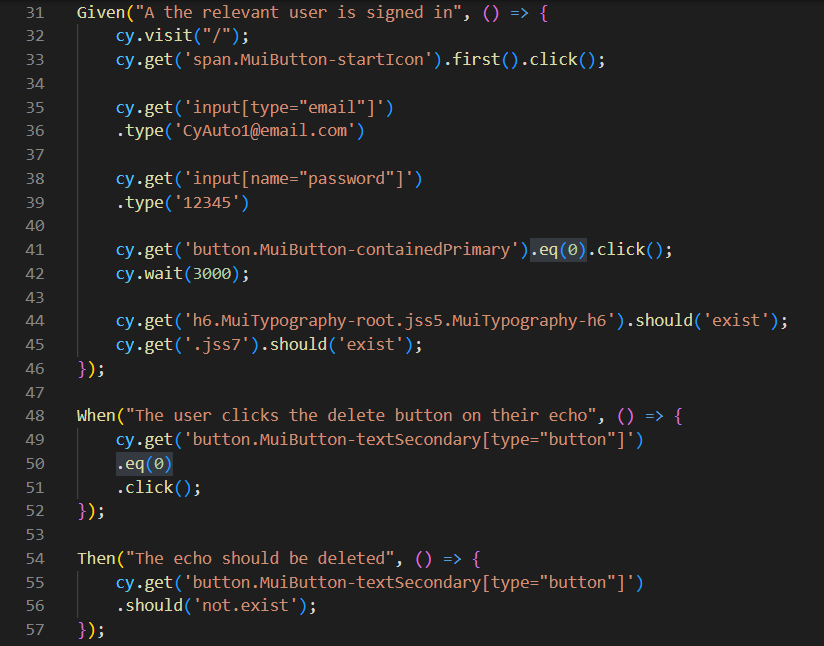
\includegraphics[width=\linewidth]{images/StepDefination}
    \caption{Step Definition}
    \label{image:StepDefination}
\end{minipage}
    \hspace{0.5cm}
    \begin{minipage}[b]{0.5\linewidth}
    \centering
   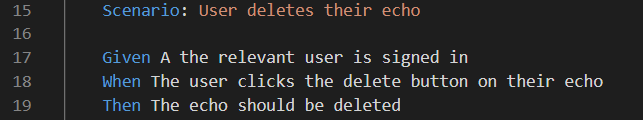
\includegraphics[width=\linewidth]{images/Feature}
    \caption{Gherkin Feature}
    \label{image:Feature}
\end{minipage}
\end{figure}

\newpage
\subsubsection{Cucumber integration with Cypress}
Cucumber is not installed with Cypress, thus it has to be installed in order to access gherkin syntax, and have it incorporated with Cypress. After Cypress is installed, Cucumber can further be added to the testing file by using these commands in the CLI, npm i @badeball/cypress-cucumber-preprocessor, this package allows programmers to define Gherkin syntax in running their Cypress tests \cite{cypress-cucumber-preprocessor}\cite{CypressPlugins}. Now Cucumber should is installed, Cypress should work using Gherkin syntax after changes to the configuration file \cite{IntergratingCucumber}.

\section{Jira Software}
Jira Software was originally created in 2002, it is a tool used by software development teams in order to track the amount of work done. Jira supports many agile methodologies which attribute as to the why it is used so widely in industry, it promotes change and ability to alter the software project \cite{fisher2013utilizing}. As mentioned above Jira uses the agile perspective to software development, for example test driven development(TDD) in which the software requirements are made into cases before code is developed in the application, thereafter the tests will assert that the application fulfils the users expectation \cite{havazik2020design}. Jira makes the above possible with, team planning where tasks are created outlining the objectives to be done during the sprint, a sprint is a duration of work normally consisting of one or two week iteration, inside the sprint, tasks called stories which are assigned to team members to be completed before the end of the sprint, during the sprint daily stand up meetings are arranged to scale how well each team member are doing with their tasks, after the sprint ends, their is a team review, and a new sprint starts again repeating the process \cite{marques2018assessing}.

\section{Kommunicate}
Kommunicate is a chat bot AI which can help a user if they need to ask questions about the application. A developer can make their own AI bot through kommunicate \cite{Kommunicate}, customize it to suit the needs of their web application, and optimize the AI to answer an questions a user might conceive while visiting the application.

\section{Platform as a Service}
Platform as a service (PaaS) refers to services that enable developers to launch their applications into a cloud-based development environment. PaaS enables an application deployment without the need to worry for operating systems or other infrastructure \cite{keller2010platform}.

\subsection{Heroku}
Heroku is a PaaS that allows developers to deliver applications online without going through the infrastructure set up \cite{WhyHeroku}. Heroku is able to run programmes across the network in virtual repositories, after which are then executed in the browser during run time \cite{danielsson2021heroku}. Such repositories can be scaled up or down based on the developers needs, for most one person projects or simple business applications only one container would be needed. 

\subsection{Hostinger}
Hostinger, another form of PaaS which allows programmers to host sites on a domain. In turn this allows the developer to choose the name of their domain after their application is built. When a developers application is built, simply drag and drop the application from the local drive into the file manager hostinger provides. After which hostinger deals with deployment of the application, then being available on the browser using the domain name that was picked upon registering the application. Features hostinger provides includes, allowing web traffic into the associated domain to exceed bandwidth where hostinger will handle it, domain name can be provided after sign up, HTTP/3 usage, and GIT support are among the most useful \cite{Hostingerfeatures}.
\chapter{System Design}
This section is concerned with how the application was made, with in-depth detail on the FrontEnd, BackEnd, architecture, deployment, how these features were made, and designed.

\section{Architecture}
The below figure \ref{image:Architecture} shows a system diagram overview architecture of the application
\begin{figure}[h!]
    \centering
    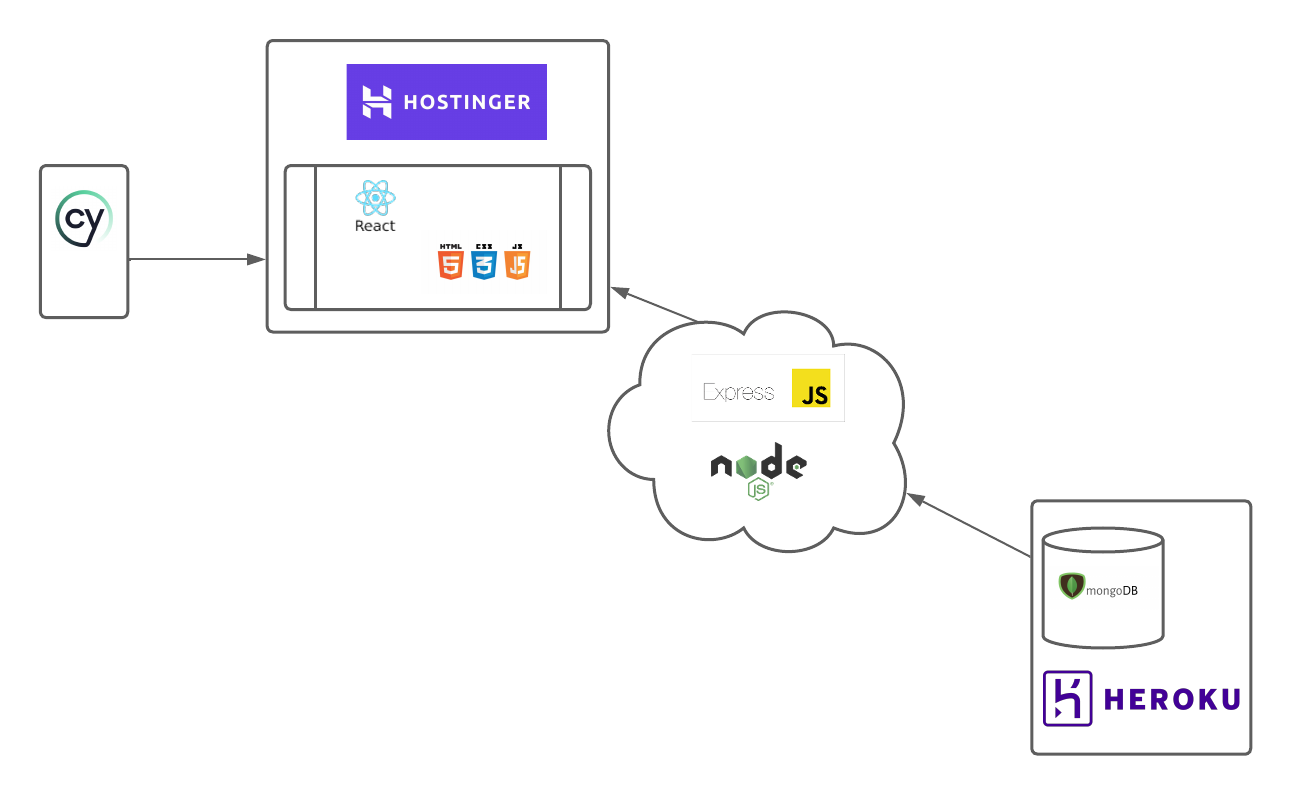
\includegraphics[width=0.8\textwidth]{images/SystemDiagram.png}
    \caption{System Architecture}
    \label{image:Architecture}
\end{figure}

\section{Front End Component Tree }
The below figure \ref{image:ReactTree} shows a high level tree of the various components in the front end of the application.
\begin{figure}[h!]
    \centering
    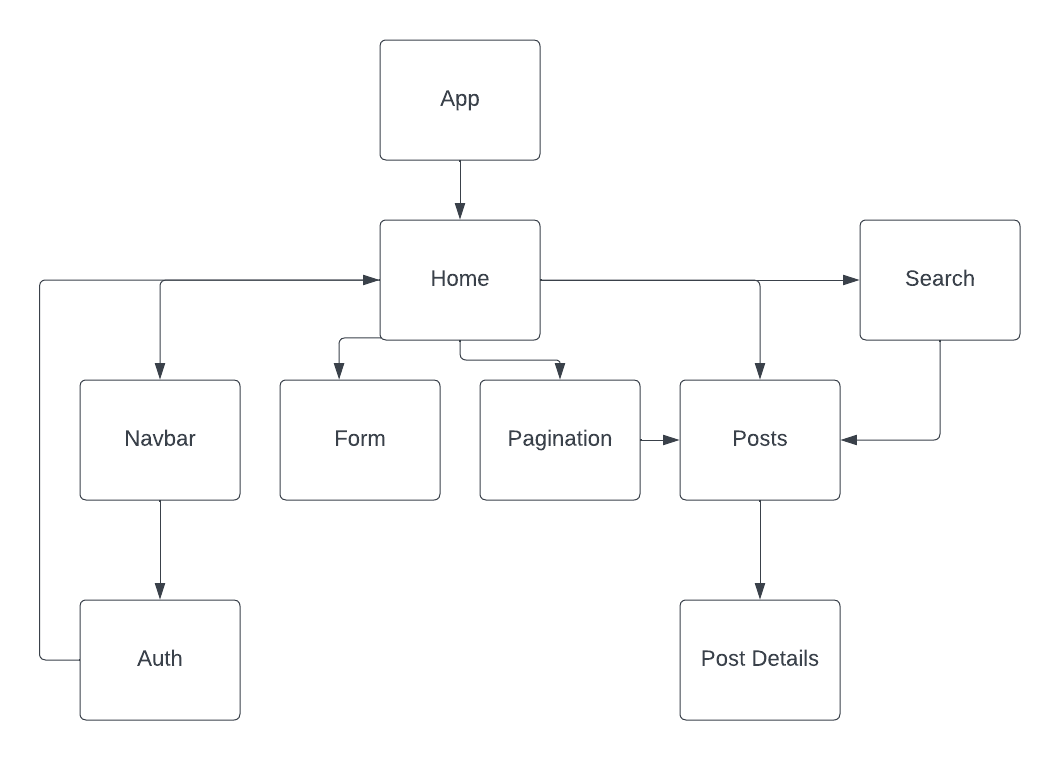
\includegraphics[width=0.8\textwidth]{images/ReactCompTree.png}
    \caption{React Component Tree}
    \label{image:ReactTree}
\end{figure}

\section{Front End Home}
The home page react component of the application encompasses rendering the home page, along with creating and viewing posts, lastly the home page is concerned with searching for a particular post.
\begin{figure}[h!]
    \centering
    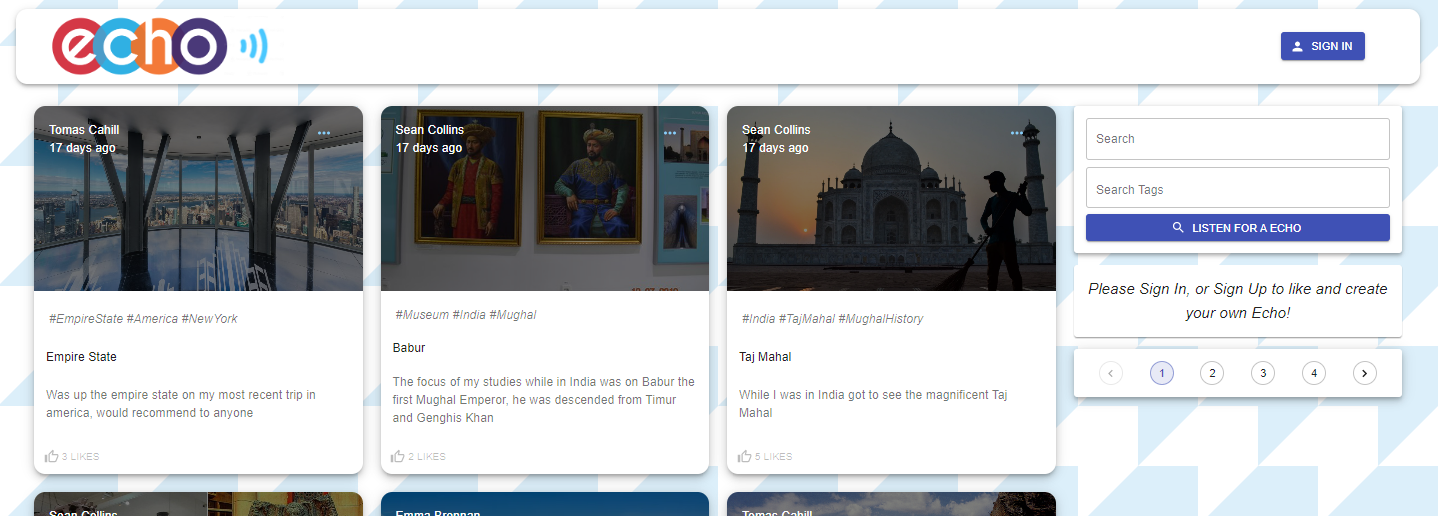
\includegraphics[width=0.7\textwidth]{images/HomePage.png}
    \caption{Home Page}
    \label{image:HomePage}
\end{figure}

\subsection{Rendering Home Page}
The home page renders various UI components such as Posts, Form, TextField, ChipInput, and Pagination using JSX syntax.  In addition it applies Material UI styles to these components using the useStyles hook.
\subsection{Search}
Search uses the useState hook from react to store the search term, or if the user uses tags instead these are stored as an array of tags using useState, subsequently useDispatch is used when the user clicks on the search button updating the URL using history.push method then displaying the desired echo. The above mentioned, dynamically search's for specific tags or search bar term based on user inputs. The tags will only be inputted into the application when the user presses the enter button.
\begin{figure}[h!]
    \centering
    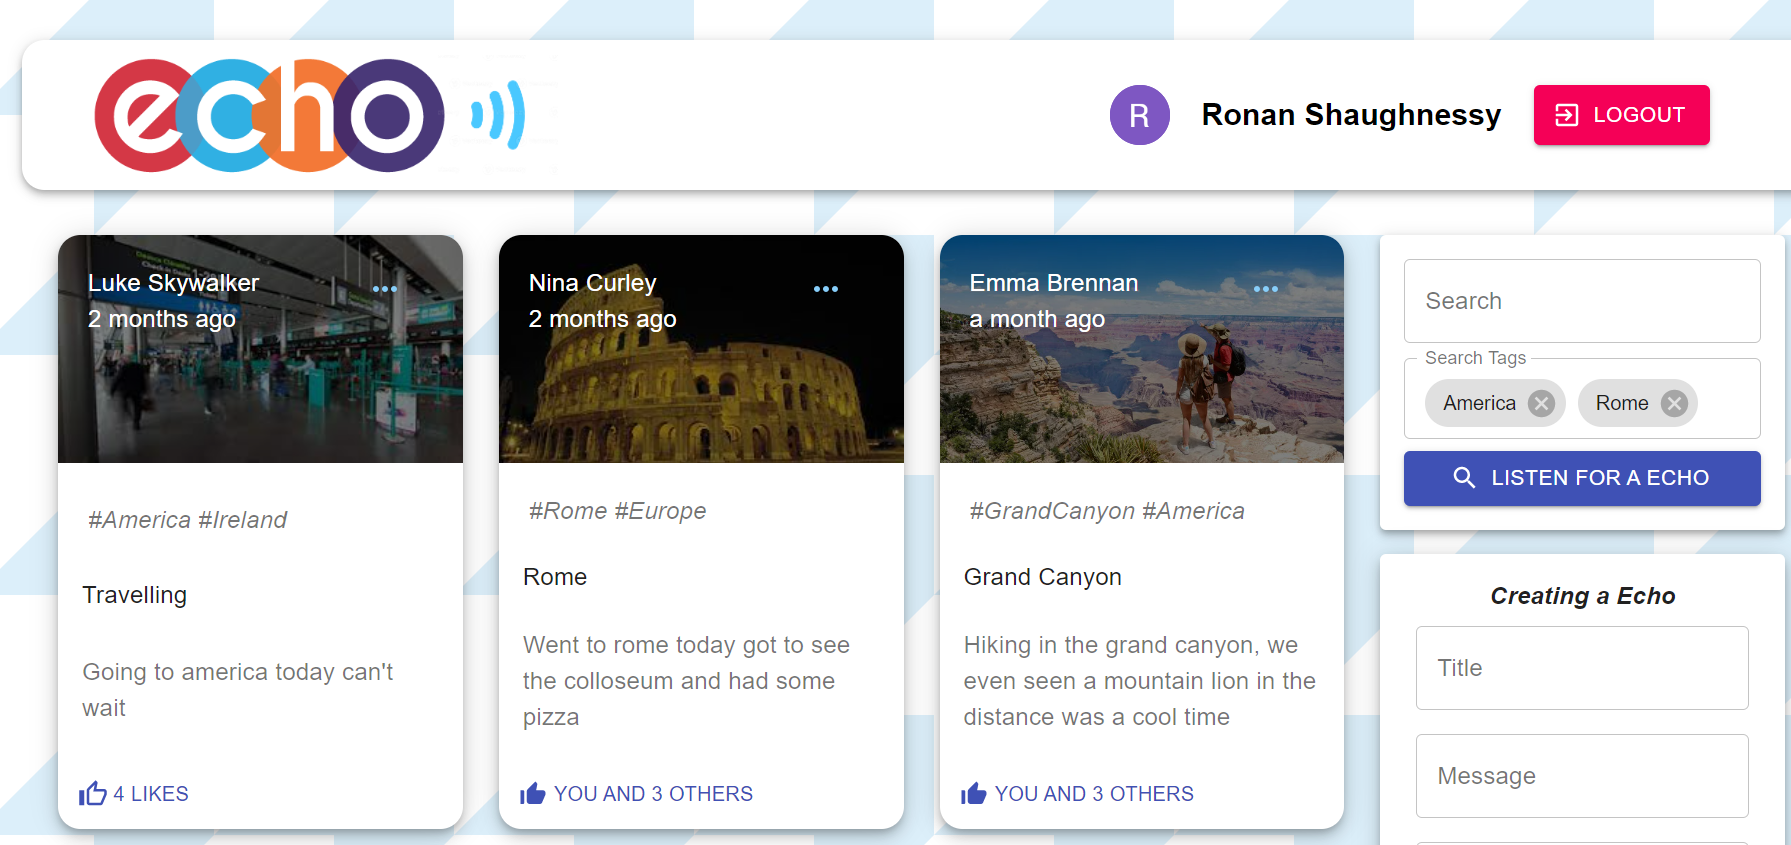
\includegraphics[width=0.7\textwidth]{images/SearchTags.png}
    \caption{Searching dynamically using tags}
    \label{image:SearchTags}
\end{figure}
\subsection{Viewing Posts}
The posts component is imported in order to view stored posts on the home page, setCurrentId is passed from posts allowing signed in users to be able to preform CRUD operations on a certain post. The setCurrentId function is defined using the useState hook. It updates the state of the currentId when the user selects a post to like or delete if applicable.

\subsection{Creating Posts}
Creating a post can be done on the home page using the form component in which the react useState is called. This hook is used to maintain its own local state for the form fields, including postData, which contains the data for the post being created. Then when the handleSubmit function is called by clicking the submit button, a createPost action uploads the new post with the data inputted in the form and adds it to the application state.

\section{Front End Form}
The form react component is responsible for creating a post once the user is signed in, the form component is imported into the home component to be rendered on the homepage.
\begin{figure}[h!]
    \centering
    \includegraphics[width=0.2\textwidth]{images/form.png}
    \caption{Form rendered on home page}
    \label{image:Form}
\end{figure}
\newline
The form only appears for a signed in user using JSON to parse local storage to see if a 'profile' is present, otherwise a message appears telling the user to sign in to create a echo. The currentID prop is used to see if the currentID is zero, if it is, then use dispatch to post the data through to the backend, when the relevant post details are filled out. Then the currentID prop is used to assign id's to the created posts, in which the id is assigned to the made post, and then  is used when a user wishes to see a post in more detail under the post details component.

\section{Front End Pagination}
The Pagination component is a simple component which allows to user to view posts on different pages by accepting a page parameter, then using the useSelector hook to access the number of pages of which this value is stored in redux. Next the useEffect hook dispatches the action getPosts, in order to recover the number of posts for the page, of which six are displayed on each page. The useEffect hook contains a page parameter to dynamically change every time the getPosts action is called, this is to facilitate posts being deleted or created.
\begin{figure}[h!]
    \centering
    \includegraphics[width=0.4\textwidth]{images/paginate.png}
    \caption{Pagination rendered on home page}
    \label{image:Paginate}
\end{figure}

\section{Front End Navbar}\label{section:navabr}
The navbar component is responsible for rendering the navbar and displaying it at the top of the application \ref{image:HomePage}. This component contains a button to sign in the user bringing the user to the auth route. When the user state is initialized using the useState hook, this parses a profile to assert if a user is signed in, then the navbar will display the signed in user and their avatar. Then when a user is signed in, the logout function can be used to dispatch a redux action to logout the user when the logout button is clicked, therein logging out the user. Finally when the user is signed in a JWT token is created, this token then expires after a specified amount of time automatically signing out the user with the useEffect hook.

\section{Front End Auth}
The auth component which can be sub typed into two forms which change if the user clicks the bottom button, launching the switchMode function to change the form to one of these options, sign in or sign up. Other functions such as the showPassword method is included, allowing the user to be able to click the eye button toggling the view of their password.

\subsection{Front End Sign Up}
Manually signing into the application can be done using the aforementioned bottom button and clicking it to switch the form, allowing the user to manually fill out their details. Error checking is preformed on this form to assert that the user cannot use an email that has already been picked, or if their passwords do not match.

\begin{figure}[h!]
    \centering
    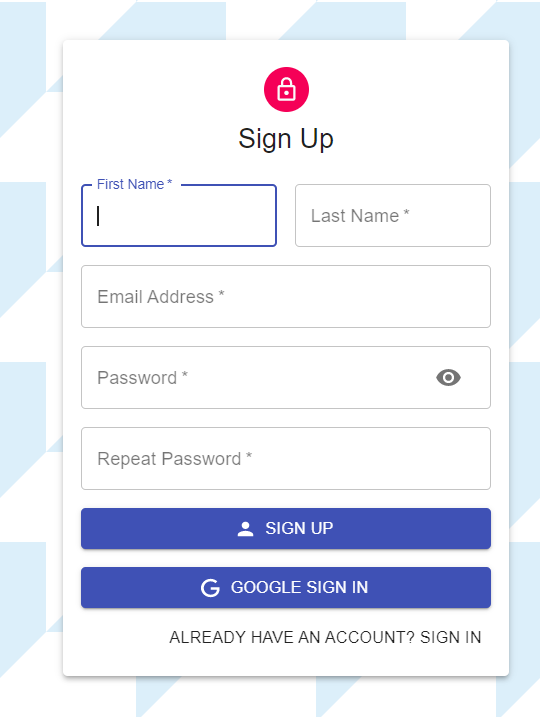
\includegraphics[width=0.5\textwidth]{images/SignUp.png}
    \caption{Sign Up Form}
    \label{image:SignUp}
\end{figure}

\newpage
\subsection{Front End Sign Up Verification Email}
Additional verification for when a user signs up to the application is used, as a welcome email appears when a user has signed up correctly. This email is sent using a BackEnd controller which can be seen here \ref{subsub:sendMail}. Below is the welcome the user receives following completion of signing up.
\begin{figure}[h!]
    \centering
    
\includegraphics[width=0.5\textwidth]{images/WelcomeEmail.png}
    \caption{Welcome email user receives}
    \label{image:WelcomeEmail}
\end{figure}

\subsection{Front End Sign In}
A user can sign into the application in two ways, one is done manually when the user signs up, filling out their details. The users data is then stored into a object called formData, this data is relayed to the backend where it is stored in the database allowing the user to sign in later. The Second option for a user to sign in is using the GoogleLogin component from react-google-login, wherein a useEffect hook is called to load the Google API client library and initialize it with the client ID, thereby signing in the user without having to manually fill out their details, this is assuming the user has a google account.

\begin{figure}[h!]
    \centering
    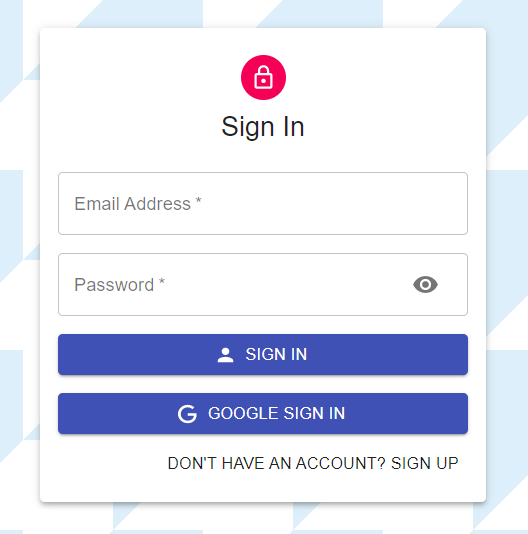
\includegraphics[width=0.5\textwidth]{images/SignIn.png}
    \caption{Sign In Form}
    \label{image:SignUp}
\end{figure}

\section{Front End Posts}
This react component manages rendering posts that the user makes in the form component as can be seen from this figure \ref{image:HomePage}. Posts lends to the search logic as there is a if statement, stating if the user has searched and no such post exists then a warning message appears. If there are posts to display to the user, a map function is called to iterate over each post and displays each of the Post components which meet the search parameters.

\subsection{Front End Post}
Inside the posts component is a sub component called post that is in control of rendering each single post and their associated content which is pulled from the database. Assuming the user is signed in, functions such as liking and deleting posts will appear for the user. These actions are controlled by using, useDispatch to make a call to redux actions to handle the like, and deleting functions. The user can also click the ellipses on the top right to view a single post in more detail.

\section{Front End Post Details}
Post details provides an in depth look at a single post, using the useSelector hook provided by react-redux library to get the state data, then rendering the aforementioned data using conditional statements. Dispatch is used to call the getPost method that gets an id parameter to fetch the particular post the user has selected from the server. Posts with similar tags will be displayed on the bottom of the page, these posts are stored as a array of recommendedPosts, which are found by filtering posts in the redux store to exclude unrelated posts, based on their tags. These recommended posts can be clicked, then using the history object from react-router-dom to route to the selected post.
\begin{figure}[h!]
    \centering
    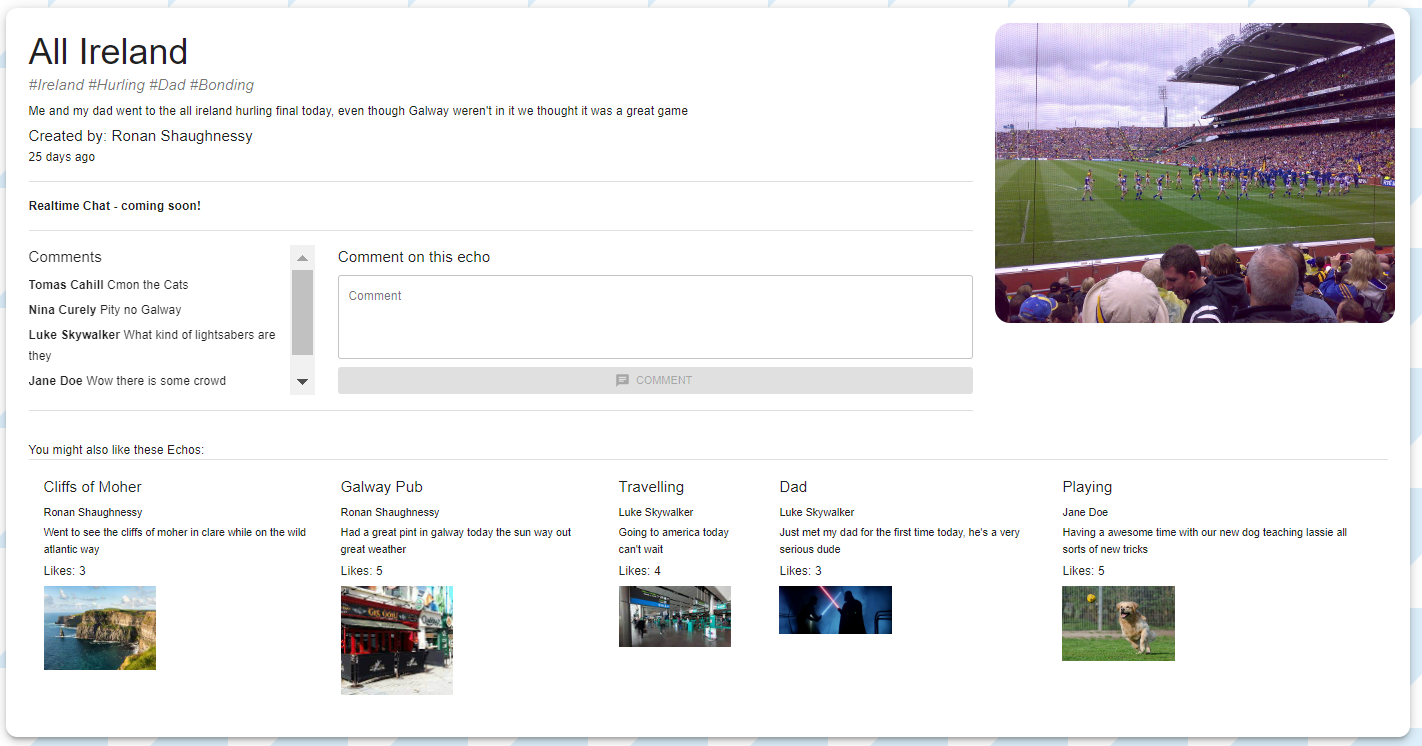
\includegraphics[width=0.5\textwidth]{images/PageDetails.png}
    \caption{Page Details}
    \label{image:PageDetails}
\end{figure}
\section{Front End Post Details Comment Section}
The comment section of the page details component is a sub component, the page details imports the comments section and renders it on the left side of the page details as seen in figure \ref{image:PageDetails}. React hooks such as useState are used to mange the comment state wherein comments are initially set to false provided there is no comments. A function called handleComment is called when the user types in a comment into the input box and clicking the comment button. This function gets the user name from local storage so their name will appear next to the comment, then using redux to dispatch an action adding the new comment to the database, finally updating the comment state with the new comment clearing the old input.

\section{Miscellaneous Front End Post Features}
Feature which don't fall into any particular category in terms of high or low level design.

\subsection{Circular Progress Bar}
If internet access is not very fast where a user is accessing the application, a circular progress bar will appear so as the user is aware that the application is loading, and that the application has not crashed.

\subsection{Kommunicate Bot}
If a user is having difficulty using the program, an AI chat bot system has been set up to answer various inquiries if the user is lost or unclear how to perform something on the site.
This was added into the indes.html file, with code provided by kommunicate to call an API which I set up containing the specifically configured bot for this application.

\section{Back End}
The back end of the application is a node.js server using express as a framework, then accessing the mongoDB database using mongoose to listen on the specified port.

\section{Back End Model View Controller}
The Model View Controller below \ref{image:MVC}, shows a high-level diagram of how the back end interacts with the application in general, where it relays information the user passes into the application, either submitting a response or adding information to the application.
\begin{figure}[h!]
    \centering
    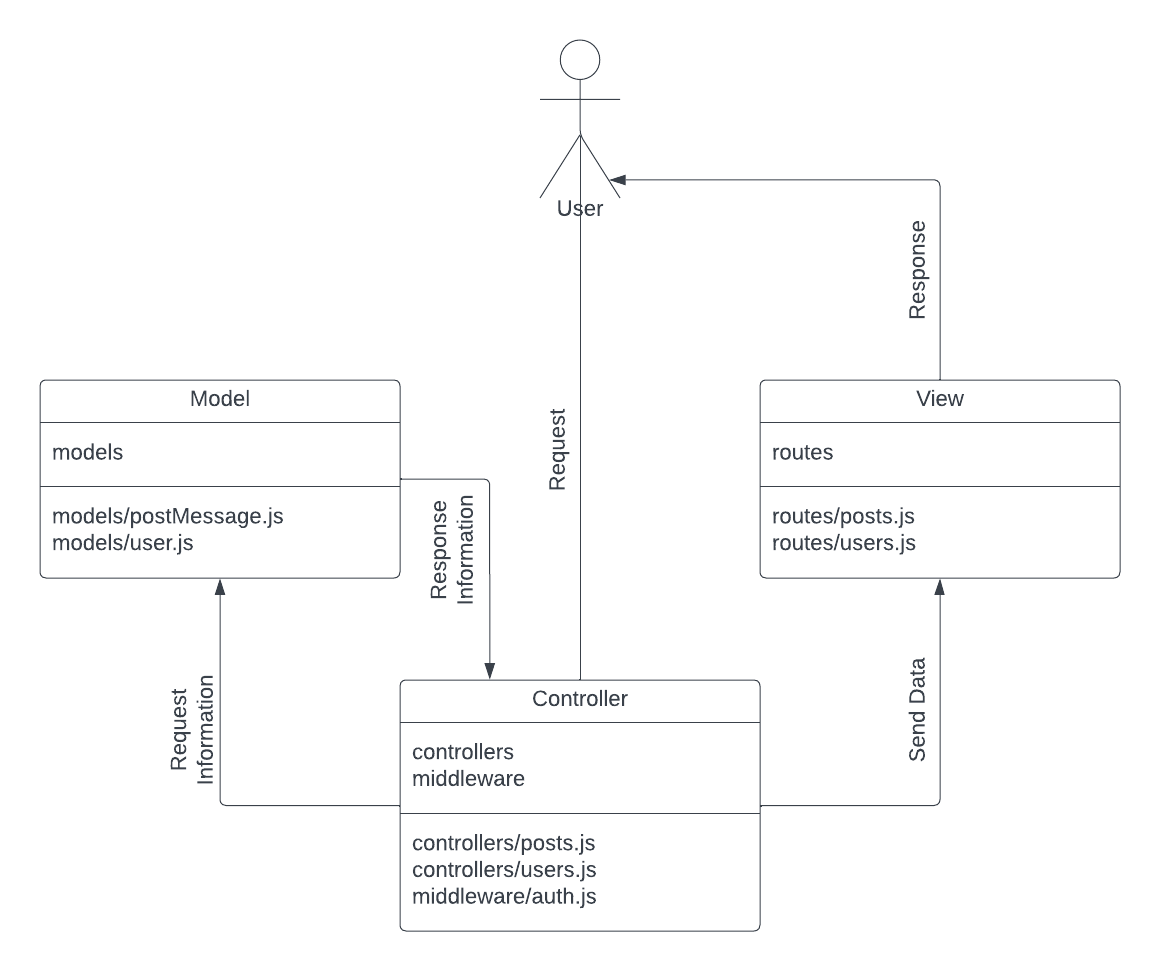
\includegraphics[width=0.8\textwidth]{images/MVC Diagram.png}
    \caption{Model View Controller Diagram}
    \label{image:MVC}
\end{figure}

\newpage
\section{Back End Controllers}
Two modules which interact as controllers for the application are the middleware, and the controllers folder modules.
\begin{figure}[h!]
    \centering
    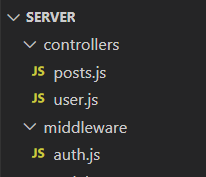
\includegraphics[width=0.2\textwidth]{images/Controllers.png}
    \caption{Controllers present in file system}
    \label{image:Controllers}
\end{figure}

\subsection{Back End post.js controller}
The post.js controller handles all routes except for the authorization routes. A router object is created at the top of the script, this allows the routes to be used in the front end of the application. A number of functions are declared in the script, for example the createPost function in which will briefly be described. The aforementioned function creates a new post with the data the user sends to the back end in the request body, wherein the function then adds the users ID, time the post was committed, and saves it to the database. A status code will then be sent to the front end of 201 for a successful request response, or 409 if there is an error. The above-stated code can be view below \ref{image:createPost}.
\begin{figure}[h!]
    \centering
    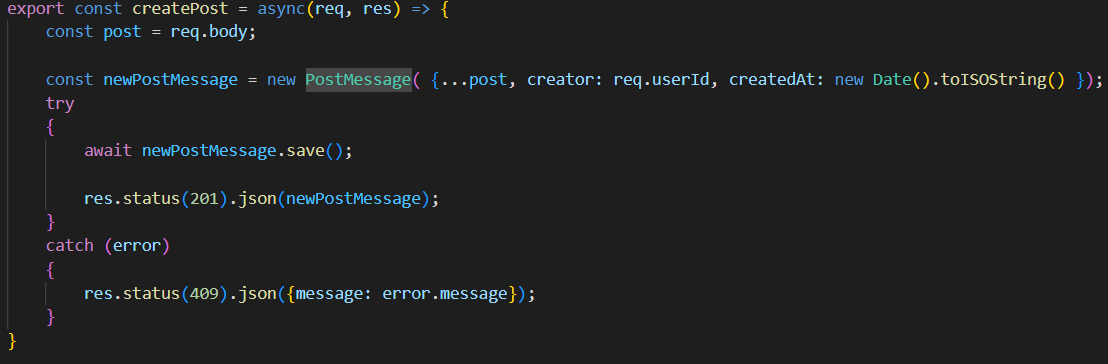
\includegraphics[width=0.8\textwidth]{images/createPost.png}
    \caption{Controller, creating a post}
    \label{image:createPost}
\end{figure}

\subsection{Back End user.js controller}
The user controller interacts in a similar way to the post controller, except in that the user controller is used as part of the authorization level of the application. Imported for this script is jsonwebtoken which is used to generate a JSON web token for authentication.
\begin{figure}[h!]
    \centering
    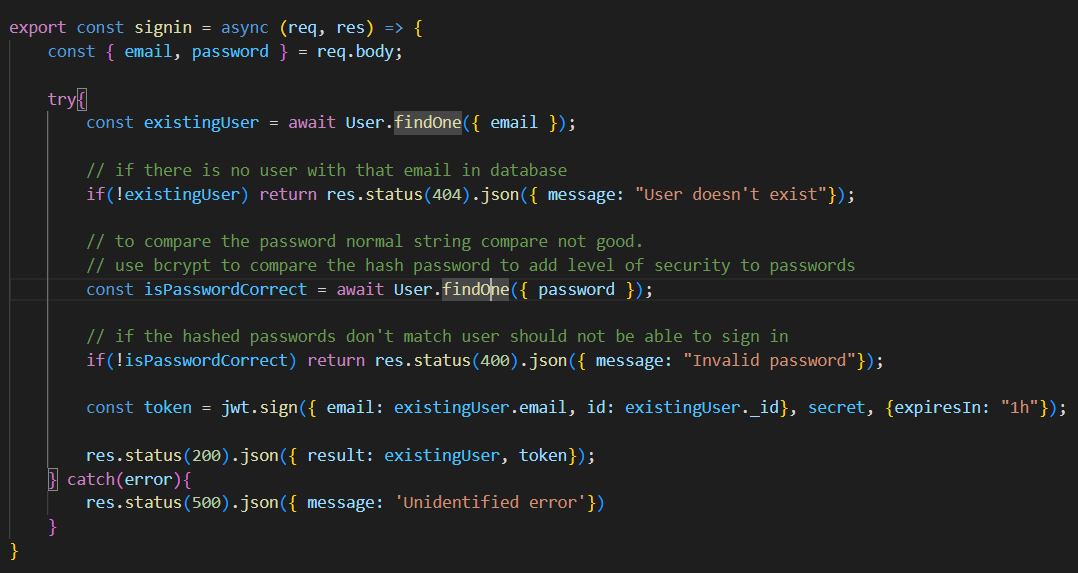
\includegraphics[width=0.8\textwidth]{images/signInCode.png}
    \caption{Controller, signing in a user}
    \label{image:signInCode}
\end{figure}
\newline
The above figure \ref{image:signInCode}, illustrates from a internal view, the programming involved in creating authorization manually. In the above function signin handles logic related to logging in. Firstly, the function pulls out the email and password the user has submitted from the request body, checking against the database using the User.findOne method to assert the email exists. If no email matches, a 404 error is returned. Secondly using the same logic as before to assert if the passwords match, if not then an error status of 400 is returned. If the password and email match, a JSON web token is created which contains the users ID and email thereby signing the user in, sending a status code of 200. The JSON web token is then configured to expire in one hour, after which the user will have to sign in again.

\subsubsection{Back End sendEmail}\label{subsub:sendMail}
The logic for sending an email from Echo's admin email to a newly registered user is handled in the function block below. The aforementioned is accomplished through the use of nodemailer library methods such as createTransport, which creates an object for sending the email i.e who it is sent by, mailOptions, which defines the details of the email to be sent, and finally sendMail, which sends the email with the prior methods filling out the details. This function is then called in the signup function block, passing in the email the user has signed up with providing it is a actual email.
\begin{figure}[h!]
    \centering
    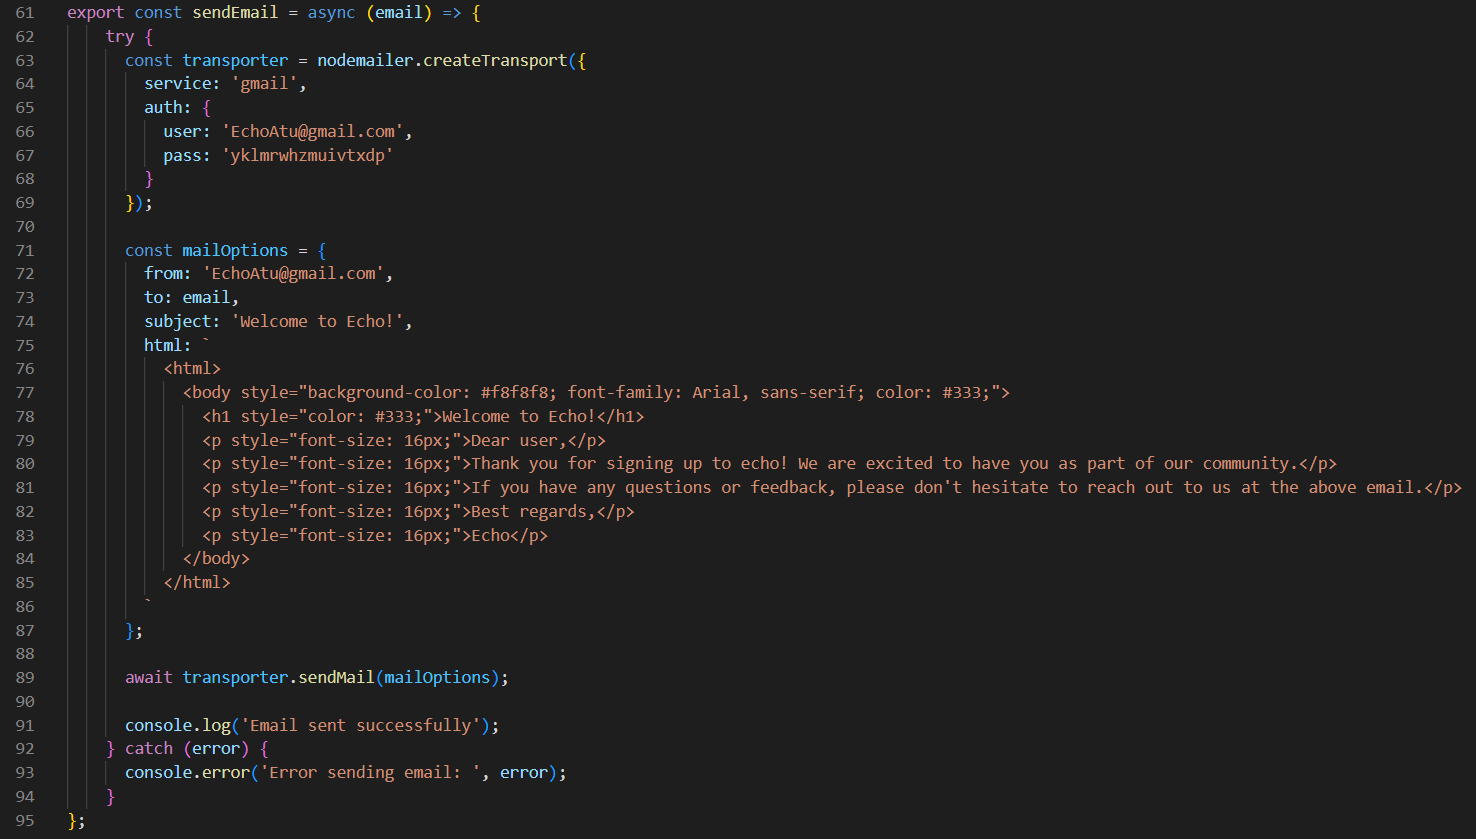
\includegraphics[width=0.5\textwidth]{images/sendEmailController.png}
    \caption{Logic to send an email to signed up user}
    \label{image:sendEmailController}
\end{figure}

\subsection{Back End auth.js middleware}
The middleware interacts with the controllers to provide an extra layer of authorization to the application, thereby passing in the middleware to the user controller, then certain functions for example liking are only available to those who sign in or up to the application. The middleware uses the jwt.verify method to assert the custom token then setting the userID property of the req object to the id property of the decoded token. If it is not a custom token the function decodes the token using the decode method and sets the userId property of the req object to the sub property of the decoded token. Lastly next is called to pass control to the user.js file in the controllers folder.

\begin{figure}[h!]
    \centering
    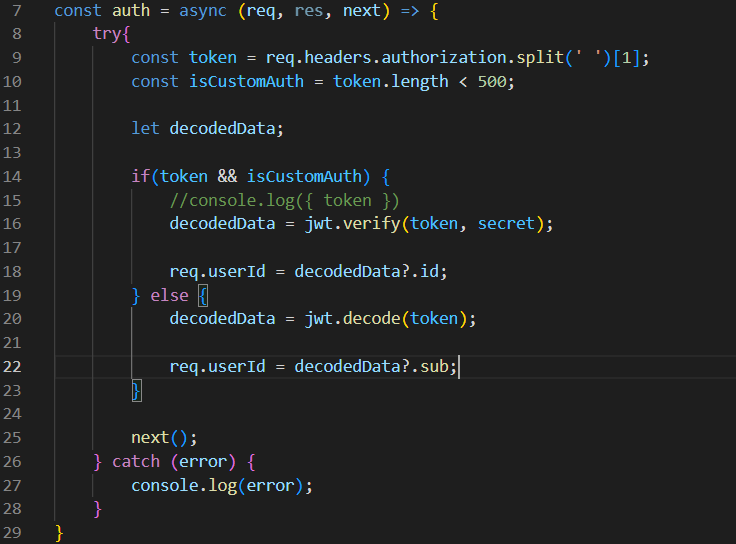
\includegraphics[width=0.5\textwidth]{images/BackEndMiddle.png}
    \caption{Logic in the auth.js middleware}
    \label{image:BackEndMiddle}
\end{figure}

\section{Back End Models}
As shown below, Mongoose is used to implement two schema that are used in the application. The schema is used when performing various CRUD operations. First and foremost, the schema function accepts various objects with a schema definition in order to establish the schema. Second, mongoose.model is used to create the collection in the database, with the collection name as the first argument and the schema as the second.
\begin{figure}[ht]
\begin{minipage}[b]{0.4\linewidth}
    \centering
    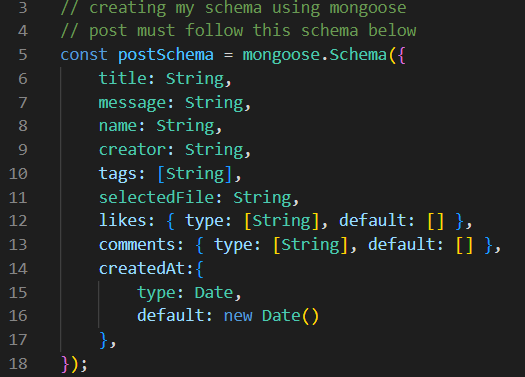
\includegraphics[width=\linewidth]{images/postMessageModel}
    \caption{Post Message Model}
\end{minipage}
    \hspace{0.5cm}
    \begin{minipage}[b]{0.5\linewidth}
    \centering
   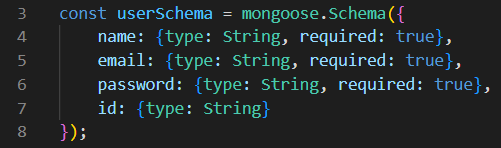
\includegraphics[width=\linewidth]{images/userModel}
    \caption{User Model}
\end{minipage}
\end{figure}

\subsection{User Model}
As previously stated, mongoose is imported into the script, and then the schema is initialized. The user must then follow the predefined schema in order to be saved properly in the database. This model in particular, is only concerned with the user signing in or up, as such the fields in this model are id, name, email, password, all of which a required fields except for id.
\subsection{Post Message Model}
Similarly to the previous model with some noticeable changes, the postMessage schema has more objects such as title, message, creator, tags, name, and selectedFile. Likes, comments, and createdAt are three distinct objects in the schema. Likes are an array of strings that are set to default, so that no post will have any likes when it is posted until a user actively likes it, at which point the like will be saved in the database. Comments work similarly to likes in that none appear in the database until a user leaves a comment on a post. Finally, the other distinct object createdAt has a field type, and date. When a user posts their echo, the default: new Date() function is used to give the exact date the post was made at, e.g. if the was made an hour ago, it will say thus, and so on.

\section{Back End Routes}
This section is concerned with the application's routes and the view section of the model view controller. The implemented scripts make use of express to handle the application's HTTP requests. The routes receive data from the controllers, then sending it to the user in a response. The majority of HTTP requests sent to the front end are get, post, patch, and delete.
\begin{figure}[ht]
\begin{minipage}[b]{0.4\linewidth}
    \centering
    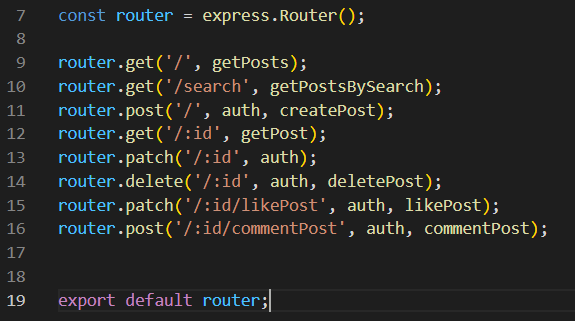
\includegraphics[width=\linewidth]{images/routePosts}
    \caption{Posts.js Routes}
\end{minipage}
    \hspace{0.5cm}
    \begin{minipage}[b]{0.5\linewidth}
    \centering
   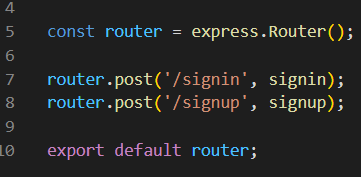
\includegraphics[width=\linewidth]{images/routeUsers}
    \caption{Users.js Routes}
\end{minipage}
\end{figure}

\subsection{Posts.js}
The applications most common response from the routing is the router.get('/', getPosts), this route handles GET requests, calls the getPosts function to retrieve a list of all posts as seen in \ref{image:HomePage}. Second, router.post('/', auth, createPost) handles a post request to the URL, requiring middleware authentication, if the authentication is successful, the user can call the createPost function from the controller. Finally, delete('/:id', auth, deletePost) handles a delete request on a specific post, asserting that the specific user has the correct id to be able to delete the post they wish to remove, this route also requires authentication.

\subsection{Users.js}
Two routing methods are present in this script strictly relating to authentication, both being HTTP post methods. Firstly router.post('/signin', signin) handles the user signing into the application, then calling the signin function from the controller, this route is used to assert the credentials through the controller. Next router.post('/signup', signup) handles the user signing up to the application, then using the signup function in the controllers to create a new user with the provided credentials

\section{Deployment}
The final phase of the the design was to deploy the application onto the internet, this was done with two hosting sites, hostinger and heroku.

\subsection{Heroku}
The server side was deployed to heroku using the heroku CLI, then the package.json script for the server was changed from start: nodemon to start:"node index.js" which makes it easier to run as npm run start is no longer required every time, and the server does not need to be run locally anymore, now there can exist two environments, so as there is always a stable version of the server online. Secondly the index script was changed to give an alert message to assert the server side is running.
\begin{figure}[h!]
    \centering
    
\includegraphics[width=0.5\textwidth]{images/deployment.png}
    \caption{Heroku Deployment}
    \label{image:deployment}
\end{figure}
\subsection{Hostinger}
In order to link the server to the client, the below code was changed from localhost:5000, to the deployed heroku url.
\begin{figure}[h!]
    \centering
    
\includegraphics[width=0.5\textwidth]{images/herokuDeploy.png}
    \caption{Connection of server to client}
    \label{image:herokuDeploy}
\end{figure}
After that, using the node command npm run build to build the client side. SSL \cite{hickman1995ssl} must be installed on hostinger, which provides the application with https security. Finally, once the application has completed the npm run build command, the build files must be dragged into the file manager on hostinger, and hostinger will build the clientside of the application, so that it can be accessed using the domain name specified when creating a website on hostinger. The application can then be seen on echoatu.com \ref{image:HomePage}.
\chapter{System Evaluation}\label{chap:Eval}
This section of the dissertation concerns evaluating the projects objectives set out in the introduction chapter \ref{chap:intro}, alongside the aforementioned, any limitations with the project, manual testing, and automated testing will also be discussed. 

\section{Cypress}
The system uses end to end testing \cite{E2ETesing} in the cypress automated testing environment, which tests the application under real time user experiences. The below are the specs which were created for the application.

\begin{figure}[h!]
    \centering
    \includegraphics[width=0.5\textwidth]{images/spec.png}
    \caption{Specs for testing the application}
    \label{image:spec}
\end{figure}

\section{Objectives}
The following are the project's objectives, which are listed in the introduction:

\begin{itemize}
    \item To create a dynamic single page application.
    \item The user can register their own account with the application.
    \item The user can sign into their own account once     	registered.
    \item A user is able to post pictures, they wish to share with their friends/family.
    \item Users can search for certain memories using taglines or memory titles.
    \item Users can send messages between each other.
    \item A user is allowed to like a picture, and comment underneath it.
    \item Users can create bio's underneath their posts.
    \item Users should be able to login to their profile and logout.
    \item Designing test scenarios to use in conjunction with cypress automated test tool. 
    \item To have a fully automated test features to verify    the application for commercial use, using test case scenarios designed.
\end{itemize}

The above will be analyzed below as to how well these objectives were completed.

\subsection{To create a dynamic single page application}
Manual testing revealed that the application is a single page application, only manual testing could be used at this level because it is difficult to determine unique ids that appear in urls such as the one below.
\begin{figure}[h!]
    \centering
    
\includegraphics[width=0.4\textwidth]{images/id.png}
    \caption{A dynamic id assigned to a post}
    \label{image:id}
\end{figure}
The key advantage of creating a single page application being the user does not have to re route multiple times to get to the page they wish to be on, also quicker loading times aiding the user experience \cite{jadhav2015single}.

\subsubsection{Other Examples of Dynamic Routing}
Other areas of the project where dynamic routing is used to make a single page application is through the below, the search bar, tags, and pagination.

\begin{figure}[ht]
\begin{minipage}[b]{0.5\linewidth}
    \centering
    
\includegraphics[width=\linewidth]{images/searchtag}
    \caption{Searching in use Dynamically}
    \label{image:searchtag}
\end{minipage}
    \hspace{0.5cm}
    \begin{minipage}[b]{0.3\linewidth}
    \centering
   
\includegraphics[width=\linewidth]{images/PaginationRoute}
    \caption{Paginate Dynamically through pages}
\end{minipage}
\end{figure}

\subsection{The user can register their own account with the application}
A user can manually create their own account by filling out the relevant form, or they can use Google's API for authorization. Manual and automated testing was recorded for manually signing up a user, but due to privacy restrictions, Google's API for signing up could only be tested manually.

\begin{figure}[h!]
    \centering
    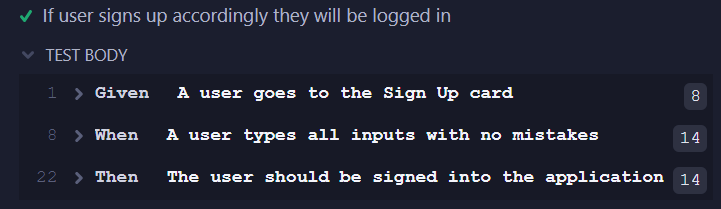
\includegraphics[width=0.4\textwidth]{images/TestPassSignUp.png}
    \caption{Specification for signing up a user manually passing}
    \label{image:TestPassSignUp}
\end{figure}

As shown above \ref{image:TestPassSignUp}, cypress is used to assert that when a user fills out the relevant fields in the authorization form, that user will be able to sign into the application, and thus a user can register to the application achieving this goal. Google's API is known to pass, but the user must have a Google account in order to use the aforementioned API, so automated testing would be ineffective. After completing this aim, testing discovered that not only was the original goal met, but it was also expanded to include two ways for a user to register with the application.

\subsubsection{Email Confirmation of sign in}
As an addition to signing up with the application, a user will be notified following successful sign up with a welcome message from the admin email. Testing of this feature was only conducted manually, setting up a mock email, after which checking their emails to see if the sendEmail api was called, which sends an email from the admin email address following sign up. The aforementioned test was successful, automating this case would not be possible due to security issues.

\subsection{The user can sign into their own account once registered}
The preceding section discusses signing up for the application, similarly signing into the application can be accomplished by using Google's API or manually entering information into the sign in form.

\begin{figure}[ht]
\begin{minipage}[b]{0.5\linewidth}
    \centering
    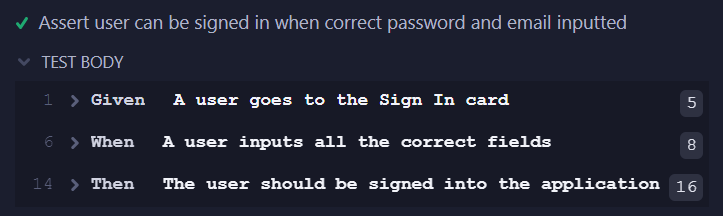
\includegraphics[width=\linewidth]{images/signinPass}
    \caption{Specification for signing in a user manually passing}
\end{minipage}
    \hspace{0.5cm}
    \begin{minipage}[b]{0.3\linewidth}
    \centering
   
\includegraphics[width=\linewidth]{images/SignedIn}
    \caption{User then signed in}
\end{minipage}
\end{figure}

Manual and automated testing has shown, that the user is able to sign into their account once it is created. Manual testing was preformed on Googles API, and on the sign in form. Automated testing was only preformed on the sign in form, not on Googles API. This objective similar to the above was also expanded upon to included Googles API for multiple ways to sign in to the application.

\subsection{A user is be able to post pictures, they wish to share with their friends/family}
If the authorization conditions are met, the user should be able to create a post and share it with all application users. In the terms of this objective, the user may also post a picture they wish to share, though this is optional, as the user may prefer not to share a picture and instead express their thoughts on current events.

\begin{figure}[ht]
\begin{minipage}[b]{0.4\linewidth}
    \centering
    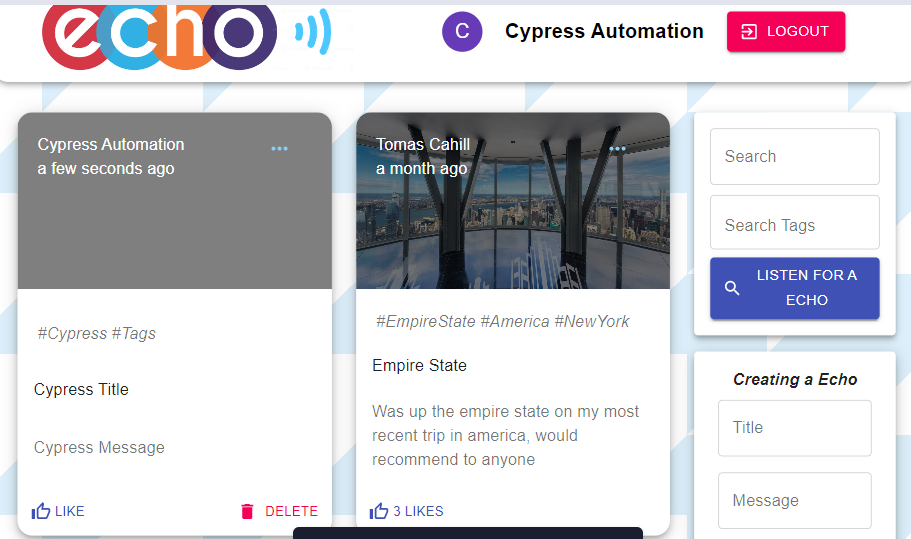
\includegraphics[width=\linewidth]{images/CreatedPost}
    \caption{Visual representation of created post}
    \label{image:CreatedPost}
\end{minipage}
    \hspace{0.5cm}
    \begin{minipage}[b]{0.4\linewidth}
    \centering
   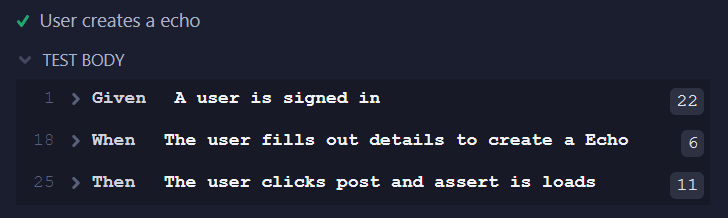
\includegraphics[width=\linewidth]{images/CreatedPostSpec}
    \caption{Automated test for user creating a post}
    \label{image:CreatedPostSpec}
\end{minipage}
\end{figure}

From the above figure \ref{image:CreatedPost}, it is shown the automated snapshot of running the specification from this figure \ref{image:CreatedPostSpec}. Due to limitations with the cypress testing tool, a picture could not be added to the post, however through manual behaviour testing preformed, it was found that a picture could be added when a file was chosen at the bottom of the creating a echo \ref{image:Form}.

\subsection{Users can search for certain memories using taglines or memory titles}
Searching in the application has been shown to be done in two ways as the requirements laid out, searching for a particular title, which is shown in this figure using a dynamic search system \ref{image:searchtag}. Moreover searching can be preformed through the use of tags \ref{image:SearchTags}.

\subsubsection{Search Testing using Title}
Carrying out automated testing on the search bar using the title of a post consisted of, inputting into the search bar what a user might search and then asserting that the right posts displayed on the screen, of which this test was found to be successful both manually and automated using cypress as can be seen below.

\begin{figure}[ht]
    \hspace{0.5cm}
    \begin{minipage}[b]{0.3\linewidth}
    \centering
   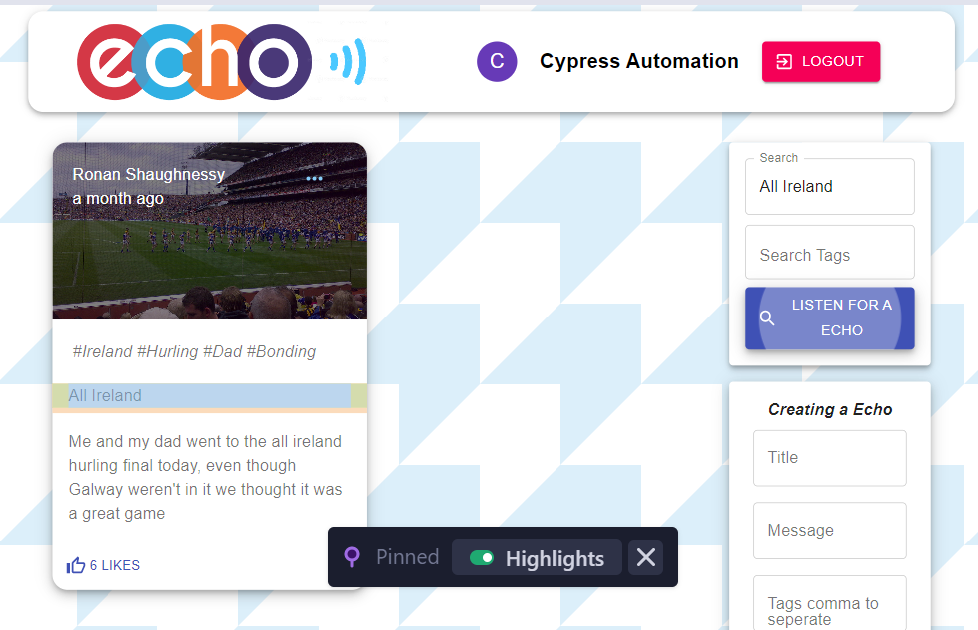
\includegraphics[width=\linewidth]{images/SearchTestSignedIn}
    \caption{Search bar test}
    \label{image:SearchTestSignedIn}
\end{minipage}
    \hspace{0.5cm}
    \begin{minipage}[b]{0.5\linewidth}
    \centering
   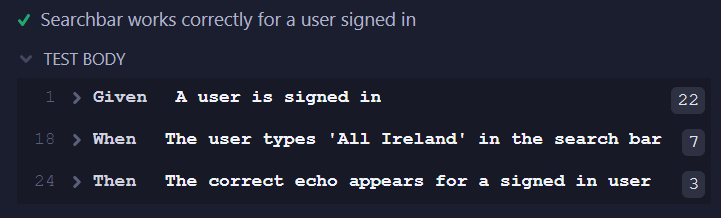
\includegraphics[width=\linewidth]{images/SignedInSeach}
    \caption{Using search bar test case}
    \label{image:SignedInSeach}
\end{minipage}
\end{figure}

\subsubsection{Search Testing using Tags}
Manual and automated testing was also preformed on tagline searches, of which searching using tags manually can be seen here \ref{image:SearchTags}. The automated version of testing can be seen below both types of testing were successful, although an element of flakiness can be seen in an automated test using tagline, which was found be attributed to the page being dynamically loaded.
\begin{figure}[ht]
    \hspace{0.5cm}
    \begin{minipage}[b]{0.3\linewidth}
    \centering
   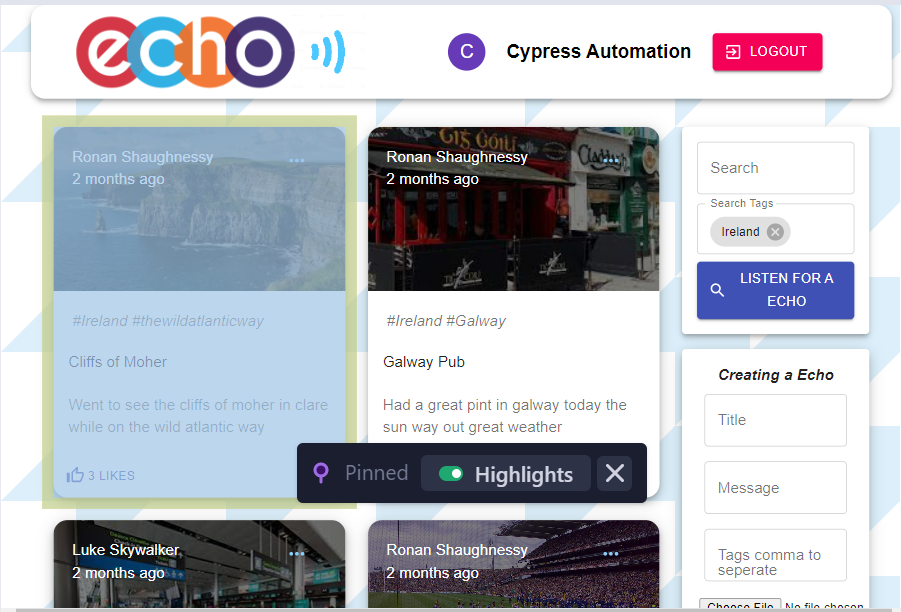
\includegraphics[width=\linewidth]{images/TagS}
    \caption{Asserting tagline working}
    \label{image:TagS}
\end{minipage}
    \hspace{0.5cm}
    \begin{minipage}[b]{0.5\linewidth}
    \centering
   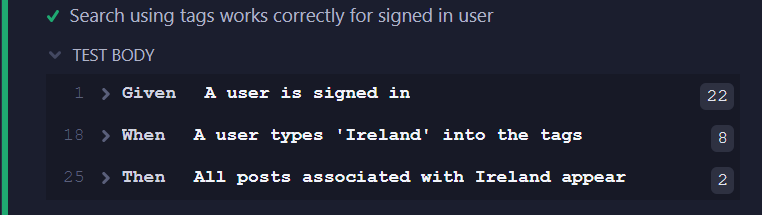
\includegraphics[width=\linewidth]{images/TagG}
    \caption{Tagline search test case}
    \label{image:TagG}
\end{minipage}
\end{figure}

\subsubsection{Search Testing using Tags and Title}
When the searching feature of the application was used to search for a title, and tags, an assertion had to be made to ensure both related posts appeared for the user. This was evaluated through the use of manual, and automated testing. Manual testing revealed that this feature was complete, and that the associated posts appears when the title and tagline inputs were filled. Automated testing was also conducted, and the results of the automated test can be seen below.
\begin{figure}[ht]
    \hspace{0.5cm}
    \begin{minipage}[b]{0.3\linewidth}
    \centering
   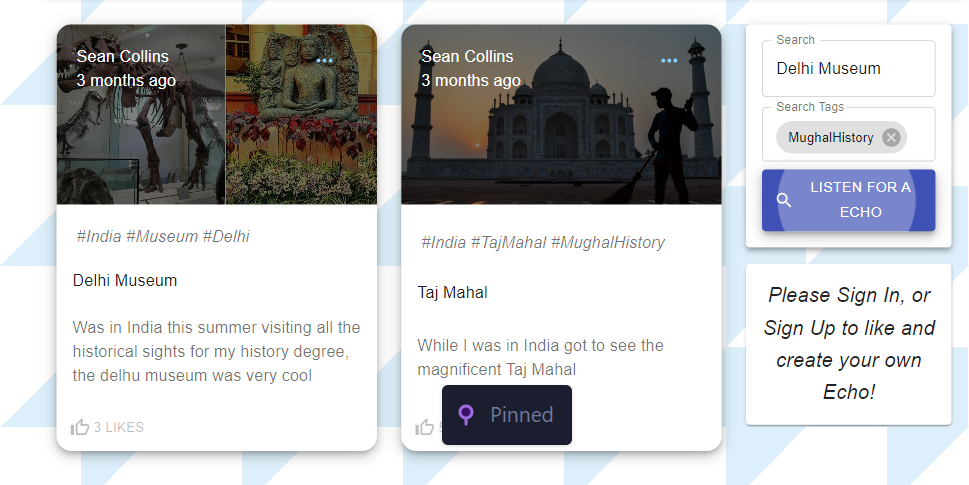
\includegraphics[width=\linewidth]{images/TagAndTitleSearch}
    \caption{Asserting tags and search title working together}
    \label{image:TagAndTitleSearch}
\end{minipage}
    \hspace{0.5cm}
    \begin{minipage}[b]{0.5\linewidth}
    \centering
   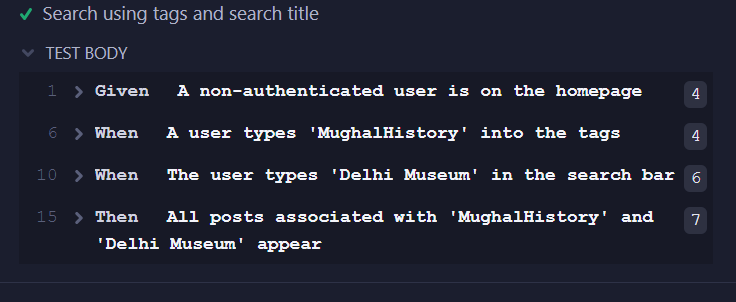
\includegraphics[width=\linewidth]{images/TagAndTitleSearchTestCase}
    \caption{Tags and search title test case}
    \label{image:TagAndTitleSearchTestCase}
\end{minipage}
\end{figure}

\subsection{Users can send messages between each other}
This objective of the project was not reached therefore, this aim is a failed component of the application. Due to time constraints this is why this part of the system was not implemented however, future iterations of the application may include messaging between users.

\subsection{A user is allowed to like a picture, and comment underneath it}
This objective passed, and has seen extensive testing, both automated and manually. This objective assumes the user is signed into the application.

\subsubsection{Liking a post}
Cypress has shown through the use of behaviour test development, that a user can like a post. In the below figure it is shown using a snapshot Cypress has taken of the application. As a result of the user clicking the like button, Cypress asserts that the application has updated the text to say "You and " then the number of likes present on the post previously, the text "You and " will only appear once a user has clicked like if they have not done so already . Manual testing was conducted prior to automated testing to ensure that the application dynamically updates to say "You and", to assert that the signed in user has liked the post.

\begin{figure}[ht]
\begin{minipage}[b]{0.4\linewidth}
    \centering
    \includegraphics[width=\linewidth]{images/LikingSignIn}
    \caption{Liking a post when signed in}
    \label{image:LikingSignIn}
\end{minipage}
    \hspace{0.5cm}
    \begin{minipage}[b]{0.4\linewidth}
    \centering
   \includegraphics[width=\linewidth]{images/LikingFeature}
    \caption{Test case for liking}
    \label{image:LikingFeature}
\end{minipage}
\end{figure}

\subsubsection{Unliking a post}
Succeeding the above test, Cypress continues to follow user behaviour as seen in this figure \ref{image:LikingFeature}, by disliking the post after liking said post. This assertion checks that when a user clicks like again, the post will then revert to its previous from e.g 3 LIKES as shown below, and will no longer have the test "You and ".

\begin{figure}[h!]
    \centering
    \includegraphics[width=0.5\textwidth]{images/Unliking.png}
    \caption{Unliking a post}
    \label{image:Unliking}
\end{figure}

\newpage
\subsubsection{Testing Comments Manually}
The user is able to comment in a post provided they are signed in. Testing was carried out manually by clicking the ellipses in the top right, which brings the user to the details of the post, of which this post screen can be seen from this figure \ref{image:PageDetails}. After which to carry out the test the comment box was clicked and a comment was inputted then the comment button was clicked, following this the comment appeared on the post thereby achieving this objective.

\subsubsection{Testing Comments using Cypress}
Cypress was employed to automatically simulate this behaviour, therein asserting that the test case passed automatically and that the objective that a user can comment on a post was met. The pretense was to type the content in the comment input box, click comment, and then assert that the username displays on the left under the comments area next to the comment which the user made.

\begin{figure}[ht]
\begin{minipage}[b]{0.4\linewidth}
    \centering
    \includegraphics[width=\linewidth]{images/CommentTest}
    \caption{Cypress automating a comment}
    \label{image:CommentTest}
\end{minipage}
    \hspace{0.5cm}
    \begin{minipage}[b]{0.4\linewidth}
    \centering
   \includegraphics[width=\linewidth]{images/CommentTestCase}
    \caption{Test case for commenting on a post}
    \label{image:CommentTestCase}
\end{minipage}
\end{figure}

\subsection{Users can create bio's underneath their posts}
Users can when creating their post as seen in this figure \ref{image:Form}, make a bio or message to go with their post. While this objective has a limitation in that when the user is writing their message or bio, the message input box does not expand with the number of words the user is using, instead the input box remains the same length and width.

\subsubsection{Bio Testing}
Testing was conducted manually and automatically, only through manual testing was the above limitation found. However as seen below in cypress the user can create a bio under their post then create the aforementioned post.

\begin{figure}[h!]
    \centering
    \includegraphics[width=0.3\textwidth]{images/MessageAuto.png}
    \caption{Cypress automatically creating a bio}
    \label{image:MessageAuto}
\end{figure}

\subsection{Users should be able to login to their profile and logout}
This objective tests the authorization of the application by asserting that a user can sign into the application, thereafter signing out if they wish.

\begin{figure}[h!]
    \centering
    \includegraphics[width=0.5\textwidth]{images/LogInandOut.png}
    \caption{Test Feature for the above objective}
    \label{image:LogInandOut}
\end{figure}

\subsubsection{Logging into a profile}
Assertions were made to test the functionality of logging in manually and automatically. First manually testing, which was done by entering in the correct inputs, then asserting that the correct user was then signed into the application, which was found to have passed as the username appears in the navbar after signing in \ref{image:CyLogIn}. Secondly the automation suite asserted that a user could be signed in, Cypress did this by asserting the correct DOM element for a username appears on screen as shown below.

\begin{figure}[h!]
    \centering
    \includegraphics[width=0.5\textwidth]{images/CyLogIn.png}
    \caption{Cypress asserting a user can log into their profile}
    \label{image:CyLogIn}
\end{figure}

\subsubsection{Logging out of a profile}
The last two steps from the feature above are done to assert that a user can log out of their profile, thereby completing this objective \ref{image:LogInandOut}. Firstly manual testing was preformed after coding was done, the finding was the logout button works, the user could log out of the application after they have signed in and have clicked the logout button. Finally, Cypress was used to take control of this test feature, automatically simulating the user's behavior. It was found to have passed as when Cypress clicks logout, the user is signed out and returned to the sign in form.

\begin{figure}[ht]
\begin{minipage}[b]{0.4\linewidth}
    \centering
    \includegraphics[width=\linewidth]{images/LogOutOne}
    \caption{Simulating clicking logging out}
    \label{image:LogOutOne}
\end{minipage}
    \hspace{0.5cm}
    \begin{minipage}[b]{0.4\linewidth}
    \centering
   \includegraphics[width=\linewidth]{images/LogOutTwo}
    \caption{After click assert sign in form appears}
    \label{image:LogOutTwo}
\end{minipage}
\end{figure}

\newpage
\subsection{Designing test scenarios to use in conjunction with cypress automated test tool}
To achieve this goal, research was conducted in order to verify the best way of implementing appropriate language for use in the test scenarios. To that end gherkin syntax was employed, in order for anyone to understand the test cases that were to be written, see this section on gherkin syntax, and how it can be used to work with cypress \ref{sec:cypress-cucumber}. Numerous test scenarios was created for the application, some of which can be seen in the above sections of this chapter, the core concept for designing these test scenarios is that anyone could understand what the test is doing, even those who do not have a software development background. These referrals are the gherkin syntax in visual studio code, \ref{image:StepDefination} the first reference is the logic code which is used to assert the authentication system works appropriately, \ref{image:Feature} the second is the plain English employed in the steps for a given scenario, the last reference is to how the gherkin format looks when it is being executed through the cypress environment \ref{image:LogInandOut}. A full list of all test scenarios can be found on GitHub \href{https://github.com/Rshocks/Final-Year-Project/tree/main/QAautomation/cypress/e2e/features}here.

\subsection{To have a fully automated test features to verify the application for commercial use, using test case scenarios designed}
Employing the above objective to support this aim, using gherkin syntax in cypress in order to format the test scenarios. Following completion of the above goal, TypeScript was used to develop the test assertions, e.g. assert that a users name appears when a user is signed in, this maintains that a user name will appear once a user is signed in, asserting the appropriate user is logged into the application. This objective was therein achieved, as the application has a fully automated test suite, allowing for changes to be made in the development of the application, then the automated tests can run against the changes made in development, in order to assert changes to the code base has not altered any other feature of the application. The below table is a result of the automated tests carried out on the application, a flaky test is a test which passes sometimes, then fails other times.

\begin{table}
\centering
    \begin{tabular}{|c|p{3cm}|c|c|c|}
    \hline
    \multicolumn{5}{|c|}{Automated Testing Results} \\
    \hline
    Feature Name & Number of Test Cases & Pass & Failed & Flaky \\
    \hline
    \hline
        authForm & 9 & 6 & 0 & 3 \\
        pageDetails & 4 & 4 & 0 & 0 \\
        routes & 9 & 9 & 0 & 0 \\
        search & 7 & 6 & 0 & 2 \\
        userActions & 6 & 6 & 0 & 0 \\
    \hline
    \end{tabular}
\caption{Cypress Automated Testing Results}
\label{table:CyAutoResults}
\end{table}

\subsubsection{Flaky Tests}\label{Flaky}
Three flaky tests were observed in the authorization feature authForm. Two of which were asserting a pop up appears on screen when the user has not filled out a relevant part of the sign in or up form. While both these tests do pass technically, it can only be seen to pass visually when the programmer visually sees the pop up appear, as it was hard to be able to assert a pop up using cypress. Secondly a flaky test was seen in signing a user up, the user signs up correctly when the spec is run for the first time, however if the spec is re run, the scenario will fail as the user is already created, this prompts the admin of the database to manually delete the user for MongoDB.

\subsubsection{Solving Flaky Tests in the Future}\label{SolveFlaky}
Solving the pop up issue so the test does not have to rely the developer visually seeing the pop up, further code must be written and documentation studied on how to assert pop up boxes. Lastly, instead of the admin removing the user from the MongoDB database, there could be a way in cypress to use a different new email when the email is already in use thereby passing the test consistently, however this could crowd the database with null users if the spec is run often.

\section{Automation Results In Cypress}
The below are the visual results of the table above \ref{table:CyAutoResults}.
\begin{figure}
        \centering
        \includegraphics[width=0.28\textwidth]{images/authFormF}
        \hfill
        \includegraphics[width=0.28\textwidth]{images/pageDetailsF}
        \hfill
        \includegraphics[width=0.28\textwidth]{images/RoutesF}
        \hfill
        \includegraphics[width=0.28\textwidth]{images/SearchF}
        \hfill
        \includegraphics[width=0.28\textwidth]{images/UserActionsF}
        \caption{Five E2E Features}
\end{figure}

\section{Limitations}\label{sec:Limit}
While most objectives were met, creating a messaging system still eludes the application, perhaps in the future using front end technology a real time chat box will be implemented into the section donated for it in the page details component, this chat box would be linked into the page details, of who is active on a certain page detail e.g users on the New York page details post will be able to chat to other users, assuming they are present on the page at the same time, after which the conversation is over the application will automatically delete it. Other limitations include the section of flaky tests covered above \ref{Flaky}. Additional limitations noted while testing the application are, to automated a spike test on the application in order to ascertain how many users the application can handle, develop a forgotten password system when the user forgets their password, and deploying the system in the app store for phone users rather than having it in the browser on a mobile.
\chapter{Conclusion}
The main idea behind developing this application was to create a software environment similar to what I might encounter after finishing my degree, such as using agile technologies to build a full stack social media application, testing the application, and creating behavior driven environment so that anyone could understand how the application should work. The application is then deployed online, and finally, a highly appealing front end look and pleasing UI were created for the application.

\section{Aims}
The purpose of creating the application, what I expected to achieve during the development of the website, and did I met my personal aims.
\begin{itemize}
    \item To build a highly pleasing front-end website, which will have a great appearance to please all who visit the application.
    \item To create multiple test scenarios, and have such scenarios fully automated using cypress.
    \item To improve my website design skills using React and JavaScript.
    \item To further my ability using automated testing.
\end{itemize}

\subsection{Aim One}
I felt I had created a stylish dynamic front end application that promotes ease of use and isn't overly cluttered, with what I consider to be a simple but elegant feel to the CSS and HTML placements of the cards, navigation bar, and form, combined with a small amount of color in the logo and background, alluding to the application not being overly cluttered.

\subsection{Aim Two}
This is my first time using behavior driven development, and I believe I designed and created test scenarios that promote ease of reading and use. I believe this is how I will develop applications from now on, writing gherkin scenarios, and incorporating such features with the development of the application, allowing testing and development to occur concurrently. When combined with cypress, it helps me achieve my fourth aim.

\subsection{Aim Three}
Throughout the course of creating this application, I have gained a much greater understanding of using JavaScript and integrating functions in JS to be used between the front end and the back end. Additionally, I am much more comfortable using React as a front end architecture, especially using this technology in conjuncture with JSX, which provides the programmer ample more control over the UI. 

\subsection{Aim Four}
Using automated testing is a real eye opener, such testing is superior, in terms of tracking metrics in which I can see what parts of the application are working as expected, and to view which sections of the application aren't working as expected. It was a great skill to pick up throughout the building of this application and I hope to carry it onward into a workplace environment using behaviour driven development.

\newpage
\section{Jira Roadmap}
A comparison of my agile roadmap, how the project occurred during the course of the year versus how I thought the project would go in my Gantt chart \ref{image:GanttChart}.
\begin{figure}[h!]
    \centering
    \includegraphics[width=0.8\textwidth]{images/AgileBoard.png}
    \caption{Agile Board}
    \label{image:AgileBoard}
\end{figure}


\section{Other Learning's}
Supplementary education I received during the course of creating the application.

\subsection{Using JSON}
I had already previously used JSON, however during the time spent on this project I used JSON Web Token(JWT) in order create a unique signature for a signed in user thereby allowing authorization to function properly.

\subsection{Creating a dynamic single page application}
Creating an SPA, which is a popular industry method for building applications that are quick and efficient.

\subsection{Using REST}
Learning more about creating a RESTful application, this would be used in conjuncture with JSON from above, and HTTP methods for declaring how the application should present the data.

\subsection{Model View Controller}
After studying the theory of MVC during my tenure at ATU, I was proud to be able to put it into practise in the back end of my project, it gave the back end substantial organisation when an addition to the application was made.

\section{Succeeding in Objectives?}
How well objectives were met was discussed in chapter \ref{chap:Eval}. However, the findings from the evaluation chapter are as follows, the system works like a dynamic single page application, authorization, search, comments and creating posts were all achieved, however creating a chat environment was not accomplished, all of the above was validated through Cypress automated test suite, and manual testing, using behaviour driven test scenarios. Limitations of the application can be seen here \ref{sec:Limit}, below is the possible future of the application.

\section{The Applications Future}
In the future I hope to add features such as having a forgotten password feature, machine learning to predict what the user wishes to search, having a real time chat in the post details section of the application, and putting the cypress tests into a pipeline like for instance Microsoft azure.

\section{Credit}
I would like to take this moment to thank my supervisor Martin Hynes who was a tremendous help throughout the project.

\chapter{Appendix}
\section{GitHub Link}
The GitHub repository for ECHO, my final year project can be found by clicking \href{https://github.com/Rshocks/Final-Year-Project}here.

\section{Installation Instructions}

\subsection{Prerequisites}
\href{https://nodejs.org/en/download}Node.js and \href{https://code.visualstudio.com/download}Visual Studio Code  will have to be installed for interaction. The deployed application can be interacted online by clicking \href{https://echoatu.com/posts}here, the testing suite must be used locally.

\subsection{Installing Test Environment}
\begin{enumerate}
\item Clone the GitHub repository to your local environment.
\item Go to the QAautomation folder, then start up a terminal environment.
\item Run npm install in the terminal.
\item After the above is finished, run npm run cypress:open, a localhost window will open, then click E2E Testing and choose a browser.
\item Click any feature you wish to test while in Spec.
\end{enumerate}

\subsection{Installing The Application Locally}
\begin{enumerate}
\item Clone the GitHub repository to your local environment.
\item Go to the client and server folders, and run a terminal environment in both.
\item Run npm install in both terminals.
\item In each terminal run npm start, at which point the application will launch on your local environment.
\end{enumerate}



%------------------------------------------------------------------------------------------------------	
% Generate the bibliography. You may have to build the document more than once before all of the
% references and processed and cited correctly.
% WARNING: Don't mess with any of the following unless you know what you are doing.
%------------------------------------------------------------------------------------------------------	
\bibliographystyle{unsrt}
\bibliography{references.bib}
\end{document}